\documentclass[11pt]{amsart}
\usepackage[T1]{fontenc}
\usepackage{lmodern}
\usepackage{amsmath,amssymb,amsthm}
\usepackage[margin=1in]{geometry}
\usepackage{booktabs}
\usepackage{longtable}
\usepackage{array}
\usepackage{enumitem}
\usepackage{xcolor}
\usepackage{tikz}
\usetikzlibrary{arrows.meta,positioning,calc}
\usepackage{url}
\usepackage[colorlinks=true,linkcolor=blue!50!black,citecolor=blue!50!black,urlcolor=blue!50!black]{hyperref}

\newtheorem{theorem}{Theorem}[section]
\newtheorem{lemma}[theorem]{Lemma}
\newtheorem{proposition}[theorem]{Proposition}
\newtheorem{corollary}[theorem]{Corollary}
\newtheorem{conjecture}[theorem]{Conjecture}
\newtheorem{problem}[theorem]{Problem}
\theoremstyle{definition}
\newtheorem{definition}[theorem]{Definition}
\newtheorem{remark}[theorem]{Remark}
\newtheorem{example}[theorem]{Example}

% Lean names, breakable at underscores and dots
\DeclareUrlCommand\lean{\urlstyle{tt}}
\renewcommand{\UrlBreaks}{\do\_\do\.\do\'\do\/}
% status tags
\newcommand{\st}[1]{\textsf{\small[#1]}}
\newcommand{\cD}{\mathcal D}
\emergencystretch=3em

\title[Gallai's conjecture and constrained Lov\'asz decompositions]{Gallai's conjecture and
constrained Lov\'asz decompositions:\\ the reduction programme, its proved parts and its frontier}
\author{Gallai project (cloud session \texttt{claude/overview})}
\date{28 November 2026}

\begin{document}

\begin{abstract}
Gallai's conjecture asserts that every connected graph on $n$ vertices decomposes into at most
$\lceil n/2\rceil$ paths. Lov\'asz proved it for graphs with at most one vertex of even degree. This paper consolidates the project's programme, which reduces the conjecture to
\emph{constrained Lov\'asz decompositions}: decompositions of a graph with at most one even vertex,
in which every odd vertex ends exactly one path, subject to conditions on the paths ending at
prescribed vertices. For every claim we state its status. ``Lean'' means formalised without
\texttt{sorry}, with only the standard axioms. ``Paper'' means proved in a project manuscript.
``Computed'' comes with its scope. ``Open'' means conjectured, with data.
\begin{itemize}[leftmargin=*]
\item \emph{The spine} (Lean). Gallai's conjecture is equivalent to two deletion tests (T1), (T2)
on $3$-connected graphs.
\item \emph{The lifts.} Each test follows from one constrained Lov\'asz decomposition, a
\emph{base}, of an auxiliary graph. There are three lifts for (T1) (triangle, forest, all-odd) and two
for (T2) (forest, floor). Every lift is reversible: for fixed data, a base exists if and only if the
test holds with a prescribed \emph{terminal} matching or forest (for the floor lift: the floor bound,
which is stronger than (T2)). Four of the five lifts are in Lean.
The all-odd lift is proved on paper only. Its converse is proved here; the converses of the two (T2)
lifts are proved in the (T2) manuscript, and in Lean for matchings, and are re-proved here.
\item \emph{Cones} (Lean). (T1) at the apex of a cone is rooted Gallai for Eulerian graphs. This
reaches the classes covered by the literature, and also roots of degree $n-2$ under a
degree condition.
\item \emph{The constrained-Lov\'asz layer.} In an all-odd graph every \emph{single} avoidance
constraint that occurs is a theorem, and so is every single sibling constraint except at a one-edge
component. The tools are separation, $L_1$, neighbour avoidance with its exact
boundary, leaf exchange, free targets and steering. With one even vertex $g$, single constraints are
\emph{reduced} to an explicit core, and proved in several special cases. The core consists of DL(1)
for $a,b\in N(g)$ with a common neighbour, and the blocked case of $L_1^*$, which follows from CLT-B1.
TRN implies Conjecture~N (Lean), N reduces DL(1) to near twins, and near twins are open.
What is open beyond that is \emph{compatibility}: several constraints in one decomposition, DL$(k)$
and its all-odd form. The obstructions are proved: universal twins, the cocktail-party barrier, the
cone over $K_{2,6}$ for forest bases, and the absence of steering schedules at roots of degree
$|J|-2$.
\item \emph{The frontier} is deletion degree $6$ with a dense neighbourhood. There two constraints
must hold at once, and every constrained vertex is adjacent to the even vertex. Lean proves that
$k$-token steering cannot reach roots of degree $|J|-2$. The asymptotic dense theorem of
Gir\~ao--Granet--K\"uhn--Osthus needs linear minimum degree and has a $o(n)$ error, so it does not
apply.
\end{itemize}
New here, besides the consolidation: the converse of the all-odd lift, with independent proofs and
checks of the (T2) converses; the all-odd lift with the root as a child of the forest, which gives (T1) at the three order-$9$ roots where every forest base fails;
and a list of disagreements between the component documents. Nothing conjectural is upgraded.
\end{abstract}

\maketitle

\setcounter{tocdepth}{1}
\tableofcontents

%======================================================================
\section{Introduction}\label{sec:intro}

\subsection{The conjecture}
All graphs are finite and simple. A \emph{path} has at least one edge and distinct vertices, and its
two \emph{ends} are distinct. A \emph{path decomposition} of $G$ is a family of paths whose edge sets
partition $E(G)$, and $p(G)$ is the least size of one.

\begin{quote}
\textbf{Gallai's conjecture.} If $G$ is connected and $|V(G)|=n$, then $p(G)\le\lceil n/2\rceil$.
\end{quote}

The conjecture was published by Lov\'asz~\cite{L68}, who proved it for graphs with at most one vertex
of even degree. It is open in general. Published partial results include the even-subgraph classes
of Pyber~\cite{Pyb} and Fan~\cite{Fan05}, maximum degree at most five (Bonamy and
Perrett~\cite{BP}), treewidth at most three~\cite{BSCL}, planar graphs, with the floor bound outside
$K_3$ and $K_5^-$~\cite{BBB}, and an asymptotic bound for dense graphs~\cite{GGKO} (\S\ref{sec:lit}).
The project's literature survey, with access levels, is
\texttt{research/notes/eulerian-gallai-literature.md}.

\subsection{Conventions}
A vertex is \emph{even} if its degree is positive and even, and \emph{odd} if its degree is odd. An
isolated vertex is neither; this is the convention of Lean's \lean{evenSet}. For a path decomposition
$\cD$, $b_\cD(v)$ is the number of path ends at $v$. $\cD$ is a \emph{parity decomposition} if
$b_\cD(v)=d(v)\bmod 2$ for every $v$. When $G$ has at most one even vertex, parity decompositions exist
(Lov\'asz~\cite{L68}; Lean \lean{lovaszStatement}, proved in \texttt{Lovasz.lean} from Fan's lemma).
They are called \emph{Lov\'asz decompositions}. $G$ is \emph{all-odd} if it has no even vertex. For an
odd vertex $v$ of a parity decomposition, $Q(v)$ is the unique path ending at $v$.

For a rooted forest $\Phi$, $p(v)$ is the parent of a non-root vertex $v$, $c(u)$ is the number of
children of $u$, and two children of the same parent are \emph{siblings}. We say that $\Phi$ is
\emph{terminal at parents} in a decomposition $\cD$ if every edge $p(v)v$ of $\Phi$ is the end edge,
at $p(v)$, of its path in $\cD$. For $T\subseteq V(H)$, a \emph{$T$-join} of $H$ is a set of edges whose
odd-degree vertices are exactly $T$.

\begin{lemma}[end count]\label{lem:count}
In every path decomposition $\cD$ of $G$, $b_\cD(v)\equiv d(v)\pmod 2$ for every $v$, and
$\sum_vb_\cD(v)=2|\cD|$. Hence if $G$ has $N$ odd vertices, then $|\cD|\ge N/2$. Equality holds if and only if
every odd vertex ends exactly one path and no other vertex ends a path, that is, if and only if $\cD$ is a
parity decomposition.
\end{lemma}

\begin{proof}
A path through $v$ uses two edges at $v$, and a path ending at $v$ uses one. So
$d(v)\equiv b_\cD(v)\pmod 2$. Each path has two ends.
\end{proof}

\subsection{Status labels}
Every statement carries one of the following labels.
\begin{itemize}[leftmargin=*]
\item \st{Lean: \textit{name}}: a declaration in \texttt{lean/GallaiLean} with no \texttt{sorry}.
Its recorded \texttt{\#print axioms} output lists only \texttt{propext}, \texttt{Classical.choice}
and \texttt{Quot.sound} (\S\ref{sec:table} gives the record and the audit for each).
\item \st{paper: \textit{source}}: proved in a project manuscript under \texttt{manuscripts/}, not
formalised. These manuscripts are unrefereed. Most have had an independent adversarial audit,
recorded in \texttt{research/audit/}.
\item \st{new}: proved here, on paper.
\item \st{computed: \textit{scope}}: exact computation, with its scope.
\item \st{open}: a conjecture or problem, with its data. \st{false}: a counterexample is known.
\item ``MR'' and ``collection'' refer to the project lead's manuscripts in \texttt{gallai/}. They are
unrefereed, and their audits are listed in \texttt{STATUS.md}~\S6a.
\end{itemize}

\subsection*{How this paper was checked}
Every statement was compared with its component manuscript and with the Lean source: the
definitions, the hypotheses and the conclusion of the named declaration, at commit \texttt{8f2c998}
of the coordinator branch. The Lean library was \emph{not} rebuilt for this paper, because the
container could not download the Lean toolchain. The axiom column of Table~\ref{tab:thms} cites the
recorded checks and audits instead. The three converses
(Propositions~\ref{prop:alloddconv}, \ref{prop:t2conv} and~\ref{prop:floorconv}) and
Example~\ref{ex:allodd} were also checked by an independent exhaustive computation
(\texttt{manuscripts/overview/scripts}; \S\ref{sec:comp}). Where components disagree, \S\ref{sec:disc}
says so.

\subsection{The programme in one paragraph}
Gallai's conjecture is equivalent to (T1) and (T2) on $3$-connected graphs
(\S\ref{sec:spine}). Each test follows from a \emph{base}: a Lov\'asz decomposition of an auxiliary
graph with at most one even vertex. Each condition of a base is a single end-path avoidance or a
distinctness of two end paths, and the lift is reversible (\S\ref{sec:lifts}). On cones, (T1) is
rooted Gallai for Eulerian graphs (\S\ref{sec:cones}). Every single avoidance that occurs in an
all-odd graph is a theorem; in a graph with one even vertex the single avoidances are reduced to an
explicit core. What is open is making several of them hold in one decomposition (\S\ref{sec:clt}). The first configuration where this cannot be avoided is deletion
degree $6$ with a dense neighbourhood (\S\ref{sec:frontier}). Figure~\ref{fig:deps} shows the
dependencies; Table~\ref{tab:thms} lists the headline theorems.

\begin{figure}[!tp]
\centering
\resizebox{\textwidth}{!}{%
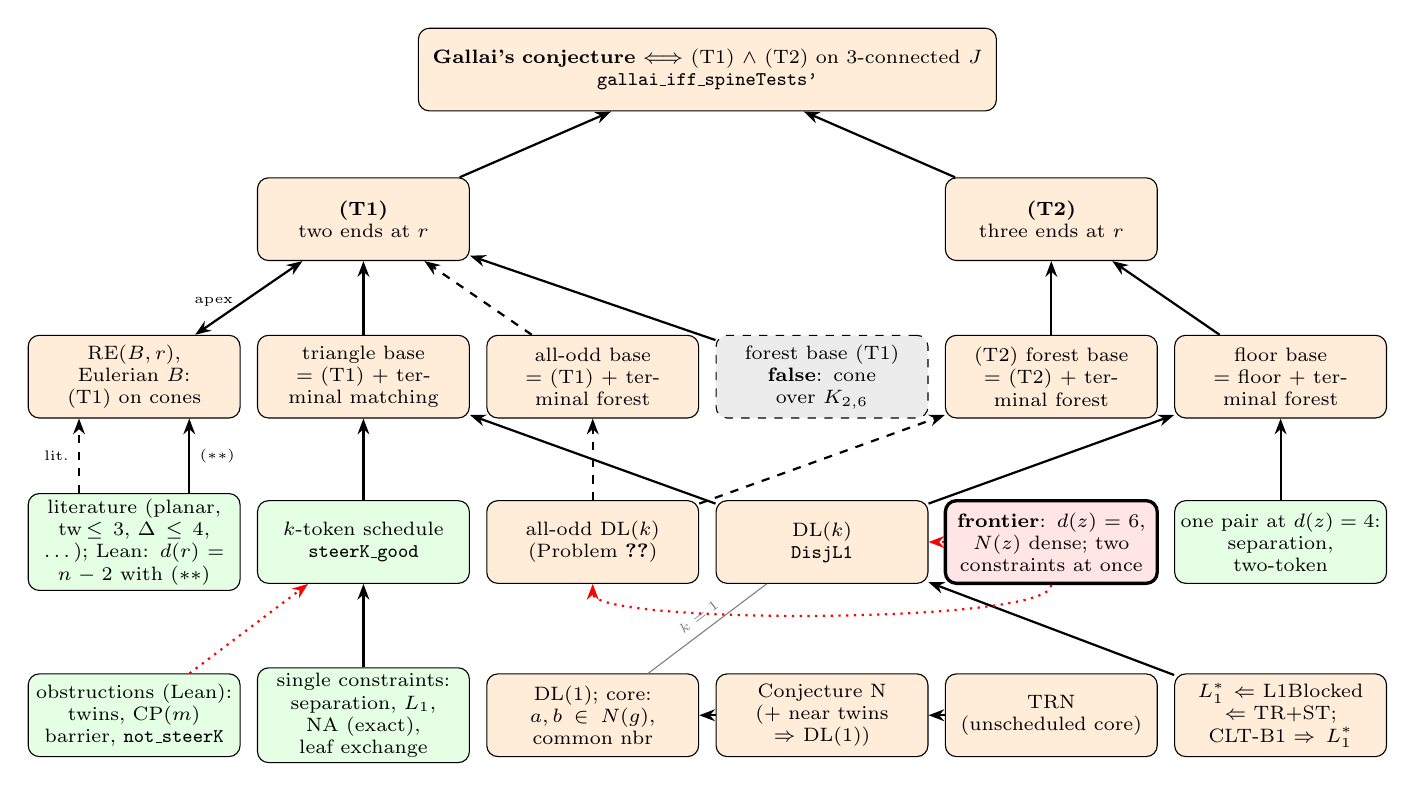
\begin{tikzpicture}[x=1.12cm,y=1cm,
  every node/.style={font=\scriptsize, align=center},
  box/.style={draw, rounded corners, text width=2.55cm, minimum height=1.05cm, inner sep=2pt},
  pr/.style={box, fill=green!10},
  op/.style={box, fill=orange!15},
  fa/.style={box, fill=gray!15, dashed},
  fr/.style={box, very thick, fill=red!10},
  L/.style={-{Stealth[length=2mm]}, thick},
  P/.style={-{Stealth[length=2mm]}, thick, dashed},
  X/.style={-{Stealth[length=2mm]}, thick, red, dotted},
  E/.style={{Stealth[length=2mm]}-{Stealth[length=2mm]}, thick},
  S/.style={thin, gray}]
% row 0
\node[op, text width=7.2cm] (G) at (0,0) {\textbf{Gallai's conjecture} $\Longleftrightarrow$ (T1) $\wedge$ (T2) on $3$-connected $J$\\ \texttt{gallai\_iff\_spineTests'}};
% row 1
\node[op] (T1) at (-3.9,-1.9) {\textbf{(T1)}\\ two ends at $r$};
\node[op] (T2) at (3.9,-1.9) {\textbf{(T2)}\\ three ends at $r$};
% row 2
\node[op] (RE) at (-6.5,-3.9) {RE$(B,r)$, Eulerian $B$:\\ (T1) on cones};
\node[op] (TB) at (-3.9,-3.9) {triangle base\\ $=$ (T1) $+$ terminal matching};
\node[op] (AO) at (-1.3,-3.9) {all-odd base\\ $=$ (T1) $+$ terminal forest};
\node[fa] (FB) at (1.3,-3.9) {forest base (T1)\\ \textbf{false}: cone over $K_{2,6}$};
\node[op] (F2) at (3.9,-3.9) {(T2) forest base\\ $=$ (T2) $+$ terminal forest};
\node[op] (FL) at (6.5,-3.9) {floor base\\ $=$ floor $+$ terminal forest};
% row 3
\node[pr] (LIT) at (-6.5,-6.0) {literature (planar, tw$\,\le3$, $\Delta\le4$, \dots); Lean: $d(r)=n-2$ with $(\ast\ast)$};
\node[pr] (SK) at (-3.9,-6.0) {$k$-token schedule\\ \texttt{steerK\_good}};
\node[op] (AODL) at (-1.3,-6.0) {all-odd DL$(k)$\\ (Problem~\ref{prob:allodd})};
\node[op] (DL) at (1.3,-6.0) {DL$(k)$\\ \texttt{DisjL1}};
\node[fr] (FR) at (3.9,-6.0) {\textbf{frontier}: $d(z)=6$, $N(z)$ dense; two constraints at once};
\node[pr] (S2) at (6.5,-6.0) {one pair at $d(z)=4$:\\ separation, two-token};
% row 4
\node[pr] (OB) at (-6.5,-8.2) {obstructions (Lean): twins, CP$(m)$ barrier, \texttt{not\_steerK}};
\node[pr] (ONE) at (-3.9,-8.2) {single constraints: separation, $L_1$, NA (exact), leaf exchange};
\node[op] (DL1) at (-1.3,-8.2) {DL(1); core:\\ $a,b\in N(g)$, common nbr};
\node[op] (N) at (1.3,-8.2) {Conjecture N\\ ($+$ near twins $\Rightarrow$ DL(1))};
\node[op] (TRN) at (3.9,-8.2) {TRN\\ (unscheduled core)};
\node[op] (L1S) at (6.5,-8.2) {$L_1^*\Leftarrow$ L1Blocked $\Leftarrow$ TR$+$ST;\\ CLT-B1 $\Rightarrow L_1^*$};
% arrows
\draw[L] (T1) -- (G); \draw[L] (T2) -- (G);
\draw[E] (RE) -- node[left, pos=0.45]{\tiny apex} (T1);
\draw[L] (TB) -- (T1);
\draw[P] (AO) -- (T1);
\draw[L] (FB) -- (T1);
\draw[L] (F2) -- (T2);
\draw[L] (FL) -- (T2);
\draw[P] ([xshift=-7mm]LIT.north) -- node[left]{\tiny lit.} ([xshift=-7mm]RE.south);
\draw[L] ([xshift=7mm]LIT.north) -- node[right]{\tiny $(\ast\ast)$} ([xshift=7mm]RE.south);
\draw[L] (SK) -- (TB);
\draw[L] (DL) -- (TB);
\draw[L] (DL) -- (FL);
\draw[P] (AODL) -- (AO);
\draw[P] (AODL) -- (F2);
\draw[L] (S2) -- (FL);
\draw[L] (ONE) -- (SK);
\draw[S] (DL1) -- node[above, sloped]{\tiny $k=1$} (DL);
\draw[P] (N) -- (DL1);
\draw[L] (TRN) -- (N);
\draw[L] (L1S) -- (DL);
\draw[X] (FR) -- (DL);
\draw[X] (FR.south) .. controls (3.9,-7.05) and (-1.3,-7.05) .. (AODL.south);
\draw[X] (OB) -- (SK);
\end{tikzpicture}}
\caption{Dependencies. Solid arrows are implications proved in Lean, dashed arrows are proved on paper,
and the double arrow is a Lean equivalence. Green boxes are proved, orange boxes are open, the grey box is
refuted, and the red box is the frontier. Dotted red arrows mark where the frontier and the obstructions
act: the frontier is the first case of DL$(2)$ and of all-odd DL$(2)$, and \texttt{not\_steerK} blocks
steering at roots of degree $|J|-2$. DL$(k)$ gives the triangle base when $M$ is connected and the floor base when no pair is a pair of
universal twins (Theorem~\ref{thm:dlboth}). The arrow from $L_1^*$ to DL$(k)$ covers only one pair with
$a\not\sim g$ or $b\not\sim g$ (direct-test1 Prop.~7.2). The one-pair theorem at $d(z)=4$ is the floor
base with one pair. The thin grey line is not an implication: it marks DL(1) as the case $k=1$ of
DL$(k)$. The box at the lower left feeds RE by a dashed arrow (the literature cases, through the Lean
leaf and double lemmas) and a solid arrow (the degree-$(n-2)$ theorem in Lean). Every base box is equivalent to its test with
terminal structure (\S\ref{sec:lifts}).}\label{fig:deps}
\end{figure}

%======================================================================
\section{The spine}\label{sec:spine}

\begin{definition}[the deletion tests; spine Def.~1.1]\label{def:tests}
Let $J$ be a graph, $z\in V(J)$ and $n=|V(J)|$.
\begin{itemize}[leftmargin=3em]
\item[(T1)] If $z$ is the only even vertex of $J$, then for every $r\in N(z)$ the graph $J-z$ has a
path decomposition into at most $(n-1)/2$ paths, at least two of which end at $r$.
\item[(T2)] For every $r\in N(z)$: if $z$ and $r$ are the only even vertices of $J$, then $J-z$ has a
path decomposition into at most $n/2$ paths with at least three ends at $r$.
\end{itemize}
\st{Lean: \lean{Test1}, \lean{Test2}; the conclusions at one root are \lean{Test1At},
\lean{Test2At}}
\end{definition}

In Lean the hypothesis ``$z$ is the only even vertex'' reads \texttt{Even (J.degree v) $\leftrightarrow$ v = z},
so degree $0$ counts as even and isolated vertices are excluded; for $3$-connected $J$ this makes no
difference. In (T1) $n$ is odd, and the even vertices of $B=J-z$ are exactly the neighbours of $z$. In (T2) $n$
is even, the even vertices of $B$ are $N(z)-r$, and $r$ is odd in $B$. In both tests the budget is the
Gallai bound $\lceil|B|/2\rceil$.

\begin{theorem}[the spine; MR Thm~114; spine Thm~1.2]\label{thm:spine}
The following are equivalent.
\begin{enumerate}[label=(\roman*)]
\item Gallai's conjecture.
\item (T1) and (T2) hold for every $3$-connected $J$ and every $z\in V(J)$.
\item (T1) and (T2) hold for every $3$-connected $J$ and every $z\in V(J)$ such that $J-z$ has no
matching cut.
\end{enumerate}
\st{Lean: \lean{gallai_iff_spineTests'}, no hypotheses}
\end{theorem}

\begin{proof}[Proof outline (spine \S\S3--7)]
(i)$\Rightarrow$(ii) uses the bridge double: Gallai's bound for two copies of $J-z$ joined at
$r$, together with the leaf at $r$ (spine Lemmas~7.1--7.2, Prop.~7.3; Lean \lean{spineTests_of_gallai}).
(ii)$\Rightarrow$(iii) is trivial. For (iii)$\Rightarrow$(i) there are five steps.
\begin{enumerate}[leftmargin=*]
\item \emph{Marked path numbers} (MR Thm~1). The marked bound on $2$-connected graphs and a three-end
condition imply Gallai, through a block transfer proved with Hall's theorem.
\item \emph{Matching cuts} (MR Thm~7). A $2$-connected graph with a matching cut satisfies the marked
bound once its smaller blocks do.
\item \emph{Theorem 59}. Two rooted assertions on $2$-connected graphs without a matching cut imply
the marked bound, order by order.
\item \emph{Separating pairs} (MR Thm~113). A component behind a separating pair whose vertices are
all odd is cut off.
\item \emph{Deletion tests} (MR Thm~114). At a smallest failure of the rooted assertions, a new vertex
$z$ joined to the even vertices and the root gives a $3$-connected $J$ on which (T1) or (T2) fails.
\end{enumerate}
Lov\'asz's theorem and Hall's theorem are the only external inputs. Both are proved in the library or
in Mathlib. Audits A1, A2 and A14 found no error in MR (A1 and A2 record expository gaps and interface items);
A15 found no mathematical error in the spine paper.
\end{proof}

\begin{remark}[grading by the deletion degree]\label{rem:grading}
$d(z)$ is even and at least $4$ in a $3$-connected $J$. Known cases:
\begin{itemize}[leftmargin=*]
\item (T1) at $d(z)=4$: two-step descent and \lean{emc_four}, Lovász and Fan only
\st{Lean: \lean{test1_deg_four}, for connected $J-z$}.
\item (T2) at $d(z)\le8$: MR Thms~123 and~128 \st{collection; audit A8}. Thm~128 rests on a replayed
computer certificate (Thm~124). It is conditional on Fan--Hou--Zhou for two seven-site shapes and on
an unquoted lemma of Chu--Fan--Zhou (A8, U1--U2).
\item (T1) at $d(z)=6$, called T(6)-i, is the first open case. It is equivalent to the floor bound
for odd-order graphs with a leaf and five even vertices (MR Thm~144, now Shaik-free).
\end{itemize}
The value of the spine is that a counterexample is forced into a rigid shape: $3$-connected, at most
two even vertices, and the difficulty concentrated at one deleted vertex and its neighbourhood. The
tests are exactly as hard as the conjecture.
\end{remark}

\begin{remark}[other formal reductions]\label{rem:other}
The library also proves Gallai from:
\begin{itemize}[leftmargin=*]
\item star-terminal decompositions \st{Lean: \lean{gallai_of_stl}};
\item a route-respecting constrained Lov\'asz decomposition RR \st{Lean: \lean{gallai_of_routeRR}};
\item the descent statements \lean{BranchBase3} \st{Lean: \lean{gallai_of_branchBase3}}.
\end{itemize}
The lifts of \S\ref{sec:lifts} are the current main line. They are uniform in $d(z)$ and do not pass
through star-terminal decompositions.
\end{remark}

%======================================================================
\section{The lifts}\label{sec:lifts}

Each lift deletes a matching or a forest $\Phi$, and possibly some edges at $z$. The result is a graph
with at most one even vertex. A Lov\'asz decomposition of it is then re-assembled into a test
decomposition by appending the edges of $\Phi$ at the ends of paths.

\subsection{Forest stepping and stripping}

\begin{lemma}[forest stepping; direct-test1 Lemma~4.1]\label{lem:step}
Let $\cD$ be a path decomposition of $K$, and let $\Phi$ be a rooted forest, edge-disjoint from $K$,
on vertices of $K$. Suppose every non-root vertex $v$ of $\Phi$ ends exactly one path $P(v)\in\cD$.
For every non-root $v$, append $p(v)v$ to $P(v)$ at its end $v$. The result is a path decomposition of
$K\cup\Phi$ into $|\cD|$ paths if and only if
\begin{enumerate}[label=(\roman*)]
\item $p(v)\notin V(P(v))$ for every non-root $v$, and
\item $P(x)\ne P(y)$ for distinct siblings $x,y$.
\end{enumerate}
In the result, $\Phi$ is terminal at parents, and $b(u)=b_\cD(u)-[u\text{ is a child}]+c(u)$.
\st{Lean: \lean{append_forest}, \lean{append_forest_ends}, the ``if'' direction, appending in
parent-first order}
\end{lemma}

\begin{proof}
The map $v\mapsto p(v)v$ is a bijection onto $E(\Phi)$. A path with ends $x\ne y$ receives at most one
edge at each end, and appends at different ends commute. Receiving $p(x)x$ alone gives a path iff
$p(x)\notin V(P)$. Receiving both $p(x)x$ and $p(y)y$ gives a path iff, in addition, $p(x)\ne p(y)$.
This is (i) and (ii). The appended edge is the end edge at $p(v)$.
\end{proof}

\begin{lemma}[stripping]\label{lem:strip} \st{new}
Let $\Phi$ be a rooted forest in $G$, and let $\cD$ be a path decomposition of $G$ in which $\Phi$ is
terminal at parents. Delete every edge of $\Phi$ from its path, and discard the paths that become empty.
The result $\cD^-$ is a path decomposition of $G-E(\Phi)$ with $|\cD^-|\le|\cD|$. If $|\cD^-|=|\cD|$,
then for every non-root $v$ the shortened path $P^-$ of the path $P\ni p(v)v$ ends at $v$ and avoids
$p(v)$, and the shortened paths of two siblings are different.
\end{lemma}

\begin{proof}
An end of $P$ carries at most one edge of $\Phi$ terminal at it, namely its end edge. So $P$ loses at
most its two end edges. If it loses both and has length $2$, say $P=x\,v\,y$, then $x=p(v)=y$, which is
impossible. So $P^-$ is empty only when $P$ is a single edge of $\Phi$. Otherwise $P^-$ is $P$ with the end
vertex $p(v)$ removed (and possibly the other end too). Since $p(v)$ occurs once on $P$, $P^-$ ends at
$v$ and avoids $p(v)$. Two siblings with parent $u$ whose edges lie on one path would make $u$ both ends
of that path.
\end{proof}

\subsection{The triangle lift}

\begin{definition}[triangle data; direct-test1 Def.~1.1]\label{def:tri}
Let $z$ be the only even vertex of $J$, with $|J|=2k+1$ and $d(z)=2m$, and let $r\in N(z)$.
\emph{Triangle data} are a vertex $w\in N(z)-r$ and a perfect matching $M_0=\{a_ib_i\}_{i<m}$ of
$N(z)-\{r,w\}$ by edges of $J$. Put $M=J-zw-\{za_i,zb_i,a_ib_i\}$. In $M$, $z$ is a leaf at $r$, $w$ is
the only even vertex, every other vertex is odd, and every Lov\'asz decomposition of $M$ has $k$ paths.
\st{Lean: \lean{TriangleData}, \lean{triM}, \lean{triM_parity}}
\end{definition}

\begin{theorem}[triangle lift; direct-test1 Thm~2.1]\label{thm:tri}
Let $d_J(r)\ge3$. If $M$ has a Lov\'asz decomposition $\cD_0$ with
\begin{equation}\label{eq:disj}
a_i\notin V(Q_0(b_i))\quad\text{or}\quad b_i\notin V(Q_0(a_i))\qquad\text{for every } i,
\end{equation}
then (T1) holds at $(J,z,r)$. \st{Lean: \lean{test1At_of_triangleBase}, every $m$}
\end{theorem}

\begin{proof}[Proof outline]
\emph{Delete $z$.} If $Q_0(z)=zr$, drop it and split a path through $r$, using
$d_{M-z}(r)=d_J(r)-1\ge2$. Otherwise trim $z$. Then $r$ ends exactly two paths, and vertex sets only
shrink. \emph{Restore $M_0$.} Append $a_ib_i$ at the end chosen by~\eqref{eq:disj}. This is
Lemma~\ref{lem:step} with one-edge components.
\end{proof}

\begin{proposition}[the converse; direct-test1 Prop.~2.2]\label{prop:triconv}
For fixed data $(r,w,M_0)$: $M$ has a Lov\'asz decomposition satisfying~\eqref{eq:disj} if and only if
$J-z$ has a decomposition into at most $k$ paths, with at least two ends at $r$, in which every edge of
$M_0$ is terminal. \st{paper; checked by audit A28 exhaustively on the $444$ data choices at order $7$, and on
$1{,}148$ data choices of random graphs of order $9$}
\end{proposition}

So the \emph{triangle base} is (T1) with a prescribed terminal matching of $N(z)-\{r,w\}$. It is a
strengthening of (T1) of terminal-matching type, not a weaker statement (A28, F3). Data exist at $r$ iff
$J[N(z)-r]$ has a matching of size $m-1$. For $d(z)=6$ this means $\nu(J[N(z)-r])\ge2$, which holds at
every root of the five dense shapes of \S\ref{sec:frontier} (direct-test1 Rem.~2.4).

\begin{conjecture}[triangle base; direct-test1 Conj.~3.1]\label{conj:tri}
In a $3$-connected $J$ with only even vertex $z$, every root with triangle data has a triangle base.
\st{open; Lean \lean{TriangleBaseConj}, \lean{test1_of_triangleBaseConj}. Computed: every root with
data of every $2$-connected $J$ of order $\le9$ ($2{,}426$ roots at $\kappa=2$, $22{,}890$ at
$\kappa\ge3$); all roots of the T(6)-i residual families ($180$, $144$, $36$) and the $48$ roots of the
E28 hard graphs; $71$ of $71$ roots at $d(z)=8$, order $13$. The $59$ failures at order $\le 9$ have
$\kappa=1$, and every failing data choice contains a pair of universal twins}
\end{conjecture}

\subsection{The forest lift}

\begin{theorem}[forest lift; direct-test1 Thm~4.2]\label{thm:forest}
Let $z$ be the only even vertex of $J$, $d_J(r)\ge3$, $w\in N(z)-r$, $T=N(z)-\{r,w\}$, and let $\Phi$ be
a forest $T$-join of $J-\{z,r\}$, rooted so that $w$ is never a child. Put $M=J-zw-zT-E(\Phi)$. Then $w$ is
the only even vertex of $M$. If $M$ has a Lov\'asz decomposition with (i) $p(v)\notin V(Q_0(v))$ for
every non-root $v$ and (ii) $Q_0(x)\ne Q_0(y)$ for siblings $x,y$, then (T1) holds at $(J,z,r)$.
\st{Lean: \lean{test1At_of_forestBase}; in Lean, $\Phi$ is a list of (child, parent) edges in
parent-first order, and acyclicity is not used}
\end{theorem}

The triangle lift is the case where $\Phi=M_0$. Choosing the root of each edge is choosing the side of
the disjunction.

\begin{proposition}[the forest converse; direct-test1 Prop.~4.3]\label{prop:forestconv}
For fixed $(r,w,\Phi)$ and rooting, the base of Theorem~\ref{thm:forest} exists if and only if $J-z$ has
a decomposition into at most $k$ paths, with at least two ends at $r$, in which $\Phi$ is terminal at
parents. \st{paper}
\end{proposition}

\begin{example}[the forest base is false; direct-test1 Ex.~4.7]\label{ex:k26}
Let $J$ be the cone over $K_{2,6}$: the hubs $r,r'$ are joined to $y_1,\dots,y_6$, and $z$ is joined to
all eight. Then $J$ is $3$-connected, $z$ is its only even vertex, $d(z)=8$ and $k=4$. At $r$ and $r'$
there is no triangle data. No choice of $w$, of a forest $T$-join and of a rooting gives a forest base,
yet (T1) holds. The same failure occurs at the root $r=0$ of \texttt{HsaAD\textasciitilde\}} (order $9$,
$d(z)=6$, $d(r)=7$). There $J[N(z)]$ is a star $K_{1,4}$ centred at $r$ plus an isolated vertex, so
$N(z)-r$ is independent; direct-test1 Ex.~4.7 says ``$N(z)$ independent'', which is not right
(\S\ref{sec:disc}). \st{paper, with a hand proof for $K_{2,6}$; computed by two independent
exhaustive searches} At order $9$ the forest base exists at $2{,}435$ of the $2{,}438$ roots without
triangle data; these three are the exceptions \st{computed}. The variant in which $\Phi$ passes through
$r$ also fails there (synthesis \S25 for the cone; A38 for \texttt{HsaAD\textasciitilde\}}). By contrast, $K_{3,4}+x_1x_2$ has no triangle data but has forest
bases at every root (direct-test1 Ex.~4.6).
\end{example}

\subsection{The all-odd lift for (T1)}\label{sec:allodd}

Here nothing at $z$ survives: $z$ is deleted and $\Phi$ is taken in $B=J-z$, with $T=N(z)$ including
$r$. The graph that remains is all-odd.

\begin{theorem}[all-odd lift]\label{thm:allodd}
Let $z$ be the only even vertex of $J$, $|J|=2k+1$, $B=J-z$ and $r\in N(z)$. Let $\Phi$ be a forest of
$B$ whose odd-degree vertices are exactly $N(z)$, and root it so that either
\begin{enumerate}[label=(\alph*)]
\item $r$ is a root, or
\item $r$ is a child with $c(r)\ge2$.
\end{enumerate}
Put $H=B-E(\Phi)$. Then $H$ is all-odd, with no isolated vertex. If $H$ has a Lov\'asz decomposition
with (i) $p(v)\notin V(Q(v))$ for every non-root $v$ and (ii) $Q(x)\ne Q(y)$ for siblings $x,y$, then
(T1) holds at $(J,z,r)$. \st{new: case (a) is the coordinator's observation in synthesis \S31 (a research note, not a
manuscript), case (b) is new here; the proof below is the first written one. Not in Lean}
\end{theorem}

\begin{proof}
\emph{Parities.} For $v\in N(z)$, $d_B(v)=d_J(v)-1$ is even and $d_\Phi(v)$ is odd, so $d_H(v)$ is odd.
For $v\notin N(z)$, $d_B(v)=d_J(v)$ is odd and $d_\Phi(v)$ is even, so $d_H(v)$ is odd. So all $2k$
vertices of $H$ are odd, and a Lov\'asz decomposition $\cD$ of $H$ has exactly $k$ paths, with one end
at every vertex (Lemma~\ref{lem:count}). \emph{Lift.} Lemma~\ref{lem:step} applies with $K=H$ and gives
a decomposition of $B$ into $k=(|J|-1)/2$ paths, in which $b(r)=1-[r\text{ is a child}]+c(r)$.
\begin{itemize}[leftmargin=*]
\item In case (a), $c(r)=d_\Phi(r)\ge1$, so $b(r)\ge2$.
\item In case (b), $b(r)=c(r)\ge2$.
\end{itemize}
This is (T1) at $r$.
\end{proof}

No hypothesis on $d(r)$ is needed, and there is no leaf to remove. In the matching case ($\Phi$ a
perfect matching of $J[N(z)]$, $r$ matched to $a_0$, case (a)), the conditions are $r\notin V(Q(a_0))$
with a fixed orientation, and the disjunction~\eqref{eq:disj} for every other pair (synthesis \S31).

\begin{proposition}[the all-odd converse]\label{prop:alloddconv} \st{new}
For a fixed forest $\Phi$ as in Theorem~\ref{thm:allodd}, with any rooting, the following are
equivalent:
\begin{enumerate}[label=(\alph*)]
\item $H$ has a Lov\'asz decomposition with (i) and (ii);
\item $B$ has a decomposition into at most $k$ paths in which $\Phi$ is terminal at parents.
\end{enumerate}
Every decomposition in (b) has at least $c(r)$ ends at $r$, and an even number of them. So in cases (a)
and (b) of Theorem~\ref{thm:allodd} it satisfies (T1) at $r$.
\end{proposition}

\begin{proof}
(a)$\Rightarrow$(b) is Lemma~\ref{lem:step}. For (b)$\Rightarrow$(a), strip $\Phi$
(Lemma~\ref{lem:strip}). The result $\cD^-$ decomposes $H$, which has $2k$ odd vertices, into at most
$k$ paths. By Lemma~\ref{lem:count}, $|\cD^-|=k=|\cD|$ and $\cD^-$ is a Lov\'asz decomposition. By
Lemma~\ref{lem:strip}, the path ending at a child $v$ avoids $p(v)$, which is (i), and siblings end
different paths, which is (ii). For the last claim, the $c(r)$ edges from $r$ to its children are
terminal at $r$ on distinct paths, and $b(r)\equiv d_B(r)\equiv0$.
\end{proof}

So the all-odd base is (T1) with a terminal forest $N(z)$-join of $J-z$. Like every lift here, it is a
terminal-structure strengthening of the test.

\begin{example}[the all-odd lift beyond the forest lift]\label{ex:allodd} \st{computed; new}
In case (a) the all-odd lift fails at the hubs of the cone over $K_{2,6}$. There are $32$ forest
$V(B)$-joins of $K_{2,6}$, and none of their $128$ rootings with $r$ a root has a base
(\texttt{k26\_alloddlift.py}, exhaustive). This confirms the caveat of synthesis~\S31. Case (b),
however, succeeds there. Label the hubs $0,1$ and the leaves $2,\dots,7$, and take
$\Phi=\{20,03,04,51,16,17\}$, with roots $2$ and $5$ and children $0,3,4,1,6,7$. Then $H=B-\Phi$ has
edges $05,06,07,12,13,14$, and
\[
\cD=\{5\,0\,6,\ 0\,7,\ 2\,1\,3,\ 1\,4\}
\]
is a Lov\'asz decomposition of $H$ with (i) and (ii). Its lift is
\[
\{5\,0\,6\,1,\ 2\,0\,7\,1,\ 2\,1\,3\,0,\ 5\,1\,4\,0\},
\]
four paths covering $K_{2,6}$ with two ends at the hub $0$ (\texttt{k26\_variant\_witness.py}; the check
by hand is immediate). At \texttt{HsaAD\textasciitilde\}}, the degree-$7$ root $0$ likewise has a base
only in case (b), and every other root has one in case (a) (\texttt{hsaad\_alloddlift.py}). With
Example~\ref{ex:k26}, Conjecture~\ref{conj:tri}'s data and the forest data at order $9$, this gives:
\emph{at order $9$, every root of every $3$-connected $J$ with exactly one even vertex has a triangle, a
forest or an all-odd base}. The scope is that of the component runs: the triangle-base run over
all roots with data, the forest run over the $2{,}438$ roots without data, and the three roots here.
Audit A38 reproduced the statement independently and exactly over all $25{,}210$ roots of the
$5{,}231$ graphs.
\end{example}

The coordinator's random runs (\texttt{research/coordinator/alloddlift.py}, matching data, case (a),
$3$-connected $J$ of orders $7$, $9$, $11$) found a base at $40$ of $40$ roots with data at $d(z)=4$,
and at $54$ of $54$ at $d(z)=6$, with no lift failure; the enumeration of Lov\'asz decompositions was
capped at $4{,}000$. \st{computed} Audit A38 found, by exact search, a case-(a) matching base at all
$8{,}340$ order-$9$ roots with $d(z)=6$ in graphs where $J[N(z)]$ has a perfect matching, including
all $1{,}546$ such roots of degree $|J|-2$. \st{computed: A38}

\subsection{The (T2) lifts}\label{sec:t2}

In (T2), $z$ and $r$ are the only even vertices of $J$, $z\sim r$, $|J|=n$ is even, and $d_J(r)\ge3$.
The leaf graph is $L=J-\{zv:v\in N(z)-r\}$, that is, $J-z$ with $z$ re-attached as a leaf at $r$.

\begin{lemma}[deletion step; Lean \lean{test2At_of_leafDecomp} for the first sentence]\label{lem:leaf2}
If $L$ has a decomposition into at most $n/2$ paths with at least two ends at $r$, then (T2) holds at
$(J,z,r)$. Conversely, (T2) gives such a decomposition: append $z$ to a path ending at $r$.
\end{lemma}

\begin{proof}
Trim $z$ from its path. If that path is $zr$, drop it instead. Then $b_{J-z}(r)$ is odd, because
$d_{J-z}(r)$ is odd, and it is at least $1$. If it is $1$, split a path through $r$, which exists since
$d_{J-z}(r)\ge3$. In every case $r$ ends at least three paths and at most $n/2$ paths are used.
\end{proof}

\begin{theorem}[(T2) forest lift; test2 Thm.~4.5]\label{thm:t2forest}
Let $T=N(z)-r$, and let $\Phi$ be a forest of $J-z$ whose odd-degree vertices are exactly $N(z)$
($r$ included), rooted so that if $r$ is a child then $c(r)\ge2$. Put $M=L-E(\Phi)=J-zT-E(\Phi)$. Then
$M$ is all-odd, with no isolated vertex, and $z$ is a leaf at $r$. If $M$ has a Lov\'asz decomposition
with (i) and (ii), then (T2) holds at $(J,z,r)$. \st{Lean: \lean{test2At_of_forestBase2},
\lean{test2_of_forestBases2}}
\end{theorem}

\begin{proof}[Proof outline]
In $M$: $z$ has degree $1$; $r$ loses the odd number $d_\Phi(r)$ of edges from an even degree; a vertex
of $T$ loses $zv$ and an odd number of $\Phi$-edges; every other vertex loses an even number. So $M$ is
all-odd on $n$ vertices, and its Lov\'asz decompositions have $n/2$ paths. Lemma~\ref{lem:step} in $L$
gives $n/2$ paths with $b(r)=1-[r\text{ is a child}]+c(r)\ge2$. Then apply Lemma~\ref{lem:leaf2}.
\end{proof}

\begin{proposition}[the (T2) forest converse]\label{prop:t2conv} \st{paper: test2 Prop.~4.6 proves
the form for $J-z$ (at least three ends at $r$, when $r$ is a root with $d_\Phi(r)=1$ or a child with
$c(r)\ge2$); the leaf-graph form for every admissible rooting is proved here. Lean for matchings:
\lean{forestBase2_matching_of_test2}}
For a fixed $\Phi$ and rooting as in Theorem~\ref{thm:t2forest}, $M$ has a Lov\'asz decomposition with
(i) and (ii) if and only if the leaf graph $L$ has a decomposition into at most $n/2$ paths in which
$\Phi$ is terminal at parents. Every such decomposition has at least two ends at $r$, so it gives (T2).
\end{proposition}

\begin{proof}
($\Rightarrow$) is Lemma~\ref{lem:step}. For ($\Leftarrow$), stripping gives a decomposition of $M$,
which has $n$ odd vertices, into at most $n/2$ paths. By Lemma~\ref{lem:count} it is a Lov\'asz
decomposition with no lost path, and (i), (ii) follow from Lemma~\ref{lem:strip}. Finally, $d_L(r)$ is
even and $r$ ends the $c(r)\ge1$ paths that carry its children's edges, so $b(r)\ge2$.
Lemma~\ref{lem:leaf2} then gives (T2).
\end{proof}

So the (T2) forest base is (T2), in the leaf form of Lemma~\ref{lem:leaf2}, with a terminal forest
$N(z)$-join.

\begin{theorem}[the floor lift; test2 Thm.~5.1, Lemma~3.1]\label{thm:floor}
Let $B$ be a graph whose vertices of even degree, degree $0$ included, are exactly $w$ and the
vertices of $T$ ($w\notin T$); then $|B|$ is odd. Let $\Phi$ be
a forest of $B$ whose odd-degree vertices are exactly $T$, rooted with $w$ never a child. If $B-E(\Phi)$
(whose only even vertex is $w$, possibly isolated) has a Lov\'asz decomposition with (i) and (ii), then
$p(B)\le(|B|-1)/2$. In the (T2) setting, take $B=J-z$, $w\in N(z)-r$ and $T=N(z)-\{r,w\}$. Then the floor
bound $p(J-z)\le(n-2)/2$ follows, and with it (T2), by splitting one path at $r$.
\st{Lean: \lean{floor_of_floorBase}, \lean{test2At_of_floorBase}, \lean{test2At_of_floor}; matching
case \lean{floor_of_matchingBase}}
\end{theorem}

\begin{proposition}[the floor converse; test2 Prop.~5.2]\label{prop:floorconv} \st{paper; the proof here is
independent. Lean for matchings: \lean{matchingFloorBase_of_terminal}}
For fixed $(w,T,\Phi)$ and rooting, the floor base exists if and only if $B$ has a decomposition into at
most $(|B|-1)/2$ paths in which $\Phi$ is terminal at parents.
\end{proposition}

\begin{proof}
($\Rightarrow$) is Lemma~\ref{lem:step}. For ($\Leftarrow$): in $B-E(\Phi)$ every vertex other than $w$ is
odd. So stripping gives a decomposition with at most $(|B|-1)/2$ paths of a graph with $|B|-1$ odd
vertices. By Lemma~\ref{lem:count} it is a Lov\'asz decomposition ($w$ ends no path) with no lost path,
and Lemma~\ref{lem:strip} gives (i) and (ii).
\end{proof}

So the floor base is the floor bound for $J-z$ with a terminal forest. The floor is strictly stronger
than (T2). It fails at every \emph{tight} instance, where $p(J-z)=n/2$. Through order $10$ there are
$20$ tight instances, and in each $J-z$ is an odd semi-clique \st{computed: test2, exhaustive}. The
floor route therefore cannot cover (T2) everywhere, and the forest lift is needed there.

\begin{theorem}[deletion degree $4$ from one pair; test2 Prop.~6.1, Cor.~6.2]\label{thm:t2d4}
Let $N(z)=\{r,w,a,b\}$ with $ab\in E$. If $(J-z)-ab$, whose only even vertex is $w$, has a Lov\'asz
decomposition with $a\notin V(Q(b))$, then (T2) holds at $(J,z,r)$. If moreover $d_J(w)\ge3$, this is the case when $a,b$ have no
common neighbour in $(J-z)-ab$ (by separation), or when $((J-z)-ab,b,\{a\})$ has a two-token schedule
(\S\ref{sec:steer}). \st{Lean: \lean{test2At_of_pairAvoid}, \lean{test2At_of_pair_farApart},
\lean{test2At_of_pair_steer2}}
\end{theorem}

\emph{Data} \st{computed; \texttt{manuscripts/test2}}:
\begin{itemize}[leftmargin=*]
\item (T2) holds at all $717{,}942$ instances with $n\le10$ (every $3$-connected $J$ with exactly two
adjacent even vertices, both orientations), and every witness was verified independently.
\item Exactly $20$ instances are tight, and they are exactly those in which $J-z$ is an odd
semi-clique (test2 \S2).
\item The (T2) forest base exists at every instance of orders $8$ and $10$. At order $10$, $4$ of the
$716{,}984$ instances need case $c(r)\ge2$ with $r$ a child; there $J-z$ is a fat theta, $K_{2,7}$ or a
relative (test2 Ex.~4.7; \texttt{forestbase2\_order10\_nonroot.txt}).
\item Theorem~\ref{thm:t2d4} settles $478$ of the $554$ instances with $d(z)=4$ that have data at order
$8$ (\texttt{dz4\_order8.txt}), and $7{,}358$ of the $7{,}467$ in the order-$10$ sample ($98.5\%$;
\path{dz4_order10_sample.txt}, two budget hits).
\end{itemize}
The statements of this subsection are those of the (T2) manuscript \texttt{manuscripts/test2} (audit
A37) and of \texttt{Test2Lift.lean}, \texttt{Test2Converse.lean}. The (T2) manuscript also records that
twin-free matching data, needed in Theorem~\ref{thm:dlboth}(b), do not always exist, even outside odd
semi-cliques.

\subsection{DL gives both tests wherever data exist}

\begin{definition}[universal twins; Lean \lean{UnivTwins}]
$a,b$ are \emph{universal twins} if $b$ lies in the component $C$ of $a$ and every vertex of
$C-\{a,b\}$ is adjacent to both.
\end{definition}

\begin{conjecture}[DL$(k)$, disjunctive avoidance; direct-test1 Conj.~7.3]\label{conj:dl}
Let $G$ have at most one even vertex. Let $(a_i,b_i)_{i\le k}$ be pairs of odd vertices, all $2k$
distinct, with $a_i\not\sim b_i$, and no pair universal twins. Then some Lov\'asz decomposition
satisfies~\eqref{eq:disj} for every $i$. \st{open; Lean \lean{DisjL1}}
\end{conjecture}

\begin{theorem}[DL $\Rightarrow$ (T1) and (T2)]\label{thm:dlboth}
Assume DL. Take data $(w,M_0)$ at $r$: $w\in N(z)-r$, and a perfect matching $M_0$ of $N(z)-\{r,w\}$ by
edges of $J-z$. Assume $d_J(r)\ge3$.
\begin{enumerate}[label=(\alph*)]
\item If $z$ is the only even vertex and the graph $M$ of Definition~\ref{def:tri} is connected, (T1)
holds at $r$. \st{Lean: \lean{test1At_of_disjL1}}
\item If $z,r$ are the only even vertices, $z\sim r$, and no pair of $M_0$ is a pair of universal twins
of $(J-z)-M_0$, then (T2) holds at $r$. The proof goes through the matching case of the floor lift
(test2 Cor.~5.3). \st{Lean: \lean{test2At_of_disjL1}}
\end{enumerate}
\end{theorem}

The data are the same in both cases, and so are the $m-1$ disjunctions. The base graphs are $M$ for
(T1) and $(J-z)-M_0$ for (T2).

%======================================================================
\section{Cones: rooted Gallai for Eulerian graphs}\label{sec:cones}

Let $B$ have even order $2k$, and let $J=B+z$ be the cone, with $z$ joined to every vertex of $B$.

\begin{proposition}[eulerian-cone Props.~2.1--2.3]\label{prop:cone}
\leavevmode
\begin{enumerate}[label=(\alph*)]
\item $z$ is the only even vertex of $J$ iff $B$ is Eulerian (every degree even) and $|B|$ is even.
\st{Lean: \lean{fullCone_onlyEven_iff}}
\item $J$ is $3$-connected iff $B$ is $2$-connected. \st{Lean: \lean{kConnected_three_fullCone_iff}}
\item (T1) at $(J,z)$ holds iff, when $B$ is Eulerian of even order, for every $r$ the graph $B$ has a
decomposition into at most $|B|/2$ paths with at least two ends at $r$. Call this RE$(B,r)$.
\st{Lean: \lean{test1_fullCone_iff}, \lean{test1At_fullCone_iff}, \lean{RootedDecomp}}
\end{enumerate}
\end{proposition}

\begin{theorem}[what the spine needs of cones; eulerian-cone Cor.~2.6]\label{thm:conespine}
\leavevmode
\begin{enumerate}[label=(\alph*)]
\item For $|B|$ even, every test at every vertex of $B+z$ holds iff RE$(B,r)$ holds for all $r$ whenever
$B$ is Eulerian. The non-apex tests are vacuous. \st{Lean: \lean{fullConeTests_iff}}
\item The spine in form (iii) implies RE for every $2$-connected Eulerian $B$ of even order without a
matching cut. \st{Lean: \lean{rootedDecomp_of_spineTestsNMC}}
\item Gallai's conjecture implies RE$(B,r)$ for every connected Eulerian $B$ of even order and every $r$
with $d(r)>0$. \st{Lean: \lean{rootedDecomp_of_gallai}}
\end{enumerate}
So Gallai $\Rightarrow$ RE $\Rightarrow$ Gallai for $2$-connected Eulerian graphs of even order.
\end{theorem}

\begin{lemma}[leaf and double; eulerian-cone Lemmas~3.1, 3.2]\label{lem:leafdbl}
Let $d_B(r)$ be even and positive. Then RE$(B,r)$ holds iff $p(B+\text{leaf at }r)\le|B|/2$
\st{Lean: \lean{rootedDecomp_iff_addLeaf}}. If $|B|$ is even and $p(B\oplus_rB)\le|B|$, where
$B\oplus_rB$ is two copies of $B$ joined by an edge between the copies of $r$, then RE$(B,r)$ holds
\st{Lean: \lean{rootedDecomp_of_dbl}}.
\end{lemma}

\begin{theorem}[RE from the literature; eulerian-cone Thm.~3.3]\label{thm:lit}
Let $B$ be a connected Eulerian graph of even order and $r\in V(B)$. Then $B$ has at most $|B|/2$ paths
with two ends at $r$ in each of the following cases.
\begin{enumerate}[label=(\alph*)]
\item $B$ is planar: Blanch\'e--Bonamy--Bonichon~\cite{BBB}, every connected planar graph except $K_3$
and $K_5^-$ decomposes into $\lfloor n/2\rfloor$ paths.
\item $\mathrm{tw}(B)\le3$: Botler--Sambinelli--Coelho--Lee~\cite{BSCL}.
\item $B$ is $2$-degenerate: Anto--Basavaraju~\cite{AB}.
\item $B$ is $K_5$-minor-free: Zhang--Liu--Hong~\cite{ZLH}, an unrefereed preprint.
\item $\Delta(B)\le4$: Bonamy--Perrett~\cite{BP} ($\Delta\le5\Rightarrow\lceil n/2\rceil$), applied to
the double.
\item $\Delta(B-r)\le3$: Botler--Sambinelli~\cite[Thm.~13]{BS}.
\item $B-r$ is a forest: Pyber's theorem, used through the restatements in~\cite{BS,BP}, because the
original~\cite{Pyb} was not accessible to the project.
\end{enumerate}
\st{paper: eulerian-cone, from the literature through Lemma~\ref{lem:leafdbl}; the statements were
checked against the sources in \texttt{research/notes/eulerian-gallai-literature.md}, and those of (a)
and (e) were re-checked for this paper on arXiv}
\end{theorem}

In (a)--(d), (f) and (g) the leaf graph has odd order and a leaf, so it is none of the listed
exceptions. The cone over $K_{2,6}$, which defeats the forest base (Example~\ref{ex:k26}), is planar and
so is covered by (a). No paper found by the project proves a rooted Eulerian statement as strong as RE
(eulerian-cone \S3).

\begin{theorem}[roots of degree $n-2$; re-tight Thm.~3.1]\label{thm:degstar}
Let $B$ have even order $n=2k\ge4$, all degrees even, and $d(r)=n-2$. Let $h_t$ be the number of
neighbours of $r$ of degree at least $2t$. Suppose that for every $3\le t\le k-1$,
\[
\lfloor h_t/2\rfloor\le k+1-t\qquad\text{or}\qquad\lfloor h_{t+1}/2\rfloor\le k+1-2t .
\]
Then $B$ has a decomposition into exactly $k$ paths with exactly two ends at $r$. No connectivity
hypothesis is needed. \st{Lean: \lean{exists_decomp_of_degStar}, \lean{rootedDecomp_of_degStar};
(T1) at the cone apex: \lean{test1At_fullCone_of_degStar}}
\end{theorem}

\begin{proof}[Proof outline]
$G=B-r$ has one even vertex, the non-neighbour $s$ of $r$. A Lov\'asz decomposition of $G$ has $k-1$
paths, whose ends pair up $N(r)$, and every $x\in N(r)$ lies on exactly $d_B(x)/2$ of them. Orient each
path from its end of larger degree to its \emph{trivial end}, the one of smaller degree. Match paths to
the trivial ends they avoid. Hall's condition with defect $2$ follows from the degree hypothesis. The
second alternative uses that a trivial end lies on its own path too. Each matched pair $(P_i,b_j)$
becomes $b_iP_ia_i\,r\,b_j$, and the at most two unmatched pieces are joined at $r$.
\end{proof}

Corollaries \st{Lean: \lean{rootedDecomp_of_few_heavy}, \lean{rootedDecomp_of_deg_le_six}}: RE holds
at $r$ if at most five neighbours of $r$ have degree at least $6$, or if $n\ge10$ and every neighbour of
$r$ has degree at most $6$. \emph{The method has a limit} (re-tight Prop.~4.1, \st{paper; A31}). If
$|E(B)|\ge2k^2-3k+4$, no Lov\'asz decomposition and orientation work. This includes the cocktail-party
graph $K_{2k}-M$ for $k\ge4$.

\emph{Data} \st{computed: eulerian-cone \S6, re-tight \S5}:
\begin{itemize}[leftmargin=*]
\item RE holds at all $300{,}540$ roots of the $30{,}054$ $2$-connected Eulerian graphs of order $10$,
and at all roots of orders $4$--$8$.
\item Of the $14{,}156$ tight roots at order $10$ ($p=n/2$ is forced by end counting), $14{,}131$ have
$d(r)=n-2$, and Theorem~\ref{thm:degstar} covers $13{,}507$ of those.
\item Conjecture UC ($p_r\le\max(\mathrm{CB},\lceil n/2\rceil-1)$ on $2$-connected $B$) holds to order
$10$ \st{open}.
\end{itemize}
In a smallest counterexample to the rooted bound over both parities, every degree-$2$ vertex other than
$r$ is an ear, and no two are twins \st{paper: eulerian-cone Thm.~5.7; Lean for the insertion step,
\lean{PathDecomp.ear_insert}}. The open cases are the even-order ear, which is of $L_1^*$/DL type, and
roots of degree $n-2$ below Theorem~\ref{thm:degstar}, which are of terminal-matching type.

\begin{remark}[why cones matter]\label{rem:cones}
On a cone every lift of \S\ref{sec:lifts} removes a $T$-join of $B$, takes a Lov\'asz decomposition and
re-appends terminal edges. So a base theorem at every root would prove rooted Gallai for $2$-connected
Eulerian graphs of even order. This is open in the literature: Chu--Wang's 2025 paper on Eulerian
graphs proves $3n/5$ under a triangle-distance condition~\cite{CW}. On cones no base statement can be
easier than RE.
\end{remark}

%======================================================================
\section{The constrained-Lov\'asz layer}\label{sec:clt}

Every base of \S\ref{sec:lifts} is a Lov\'asz decomposition of a graph with at most one even vertex
$g$, subject to end-path conditions. This section lists what is proved about such conditions, what is
open, and the obstructions.

\subsection{Tools}
\begin{lemma}[Fan's lemma with vertex sets; route-descent Lemma~2.2, after Fan~\cite{Fan05}]\label{lem:fan}
Let $\cD$ decompose $K$, $t\ne u$, $tu\notin E(K)$, and suppose $b_\cD(t)$ is larger than the number of
neighbours $x$ of $u$ with $b_\cD(x)=0$. Then $K+tu$ has a decomposition $\cD^+$ with $|\cD^+|=|\cD|$,
$b_{\cD^+}=b_\cD-\mathbf 1_t+\mathbf 1_u$, and a bijection $\cD\to\cD^+$ that keeps vertex sets, except
that one path gains $u$ \st{paper}. Lean proves the containment form: every path of $\cD^+$ lies in a
path of $\cD$ plus $u$ \st{Lean: \lean{fan_single_supp}}; this is what the applications use. The end-path form (clt Thm.~5.1: ends outside
$\{u,v\}\cup N(u)$ are kept) is \st{Lean: \lean{fan_single_track}}.
\end{lemma}

Vertex sets are what Lov\'asz's induction preserves. A condition ``no path contains both $c$ and $a$'' is
therefore carried through every Fan step whose target is not $c$ or $a$. Hanging a leaf $\ell$ at $y$
turns ``$Q(y)$ avoids $x$'' into ``no path contains both $\ell$ and $x$''. This \emph{leaf trick} is
behind $L_1$, NA and steering.

\subsection{Proved single-constraint theorems}

\begin{theorem}[separation; route-descent Thm.~6.1]\label{thm:sep}
If $K$ has at most one even vertex and $X$ is \emph{packed} (pairwise at distance at least $3$), then some
Lov\'asz decomposition has every path meeting $X$ at most once. \st{Lean: \lean{separation_set},
\lean{separation}, \lean{lovasz_avoid}}
\end{theorem}

\begin{theorem}[$L_1$; route-descent Thm.~6.3]\label{thm:L1}
Let $F$ be all-odd, $c$ odd, and $Y$ packed with $Y\cap N[c]=\emptyset$. Then some Lov\'asz decomposition
meets $Y$ at most once per path and has $Q(c)\cap Y=\emptyset$. In particular $Q(c)$ can avoid any single
$a\not\sim c$. \st{Lean: \lean{lovasz_avoid_set}, \lean{lovasz_avoid_nonadj}}
\end{theorem}

\begin{proof}[Proof idea]
Hang a leaf at $c$. Then $c$ is the only even vertex, and $\{\ell\}\cup Y$ is packed. Apply separation,
and delete the leaf.
\end{proof}

So in an all-odd graph a single disjunction~\eqref{eq:disj} always holds, with no exception
\st{Lean: \lean{disjL1_one_allOdd}}. Every avoidance condition (i) of the all-odd lift, taken alone, is
a theorem: $p(v)\not\sim v$ in $H$, since the only edge $p(v)v$ is in $\Phi$. A sibling condition (ii)
alone is a theorem too, by $L_1$ when $x\not\sim y$ and by Lemma~\ref{lem:np} below when $x\sim y$,
unless $x$ and $y$ form a one-edge component of $H$.

\begin{theorem}[NA, set form, exact boundary; na Thm.~1.2, Cors.~1.3, 1.5, Thm.~6.1]\label{thm:na}
Let $G$ be all-odd, $Y$ packed, and $y\notin Y$ odd. Some Lov\'asz decomposition meets $Y$ at most once
per path and has $Q(y)\cap Y=\emptyset$ \emph{if and only if} the component of $y$ in $G-Y$ contains a vertex
of positive degree with no neighbour in $Y$. For $Y=\{x\}$: $Q(y)$ can avoid $x$ iff the component of $y$
in $G-x$ contains a vertex not adjacent to $x$. In particular, if $x\sim y$ and $y$ has a neighbour
$w\ne x$ with $w\not\sim x$, then $Q(y)$ can avoid $x$ (Conjecture NA of conj-n).
\st{Lean: \lean{avoid_packed_of_reach}, \lean{avoid_packed_iff_reach}, \lean{avoid_iff_reach},
\lean{neighbourAvoidOn}}
\end{theorem}

\begin{proof}[Proof idea]
Hang a leaf $\ell$ at $y$, so that $y$ is the only even vertex. Run Lov\'asz's Case I from $y$ with targets
outside $\{\ell\}\cup Y$; Fan's lemma with vertex sets carries the condition back. A parity-trail lemma
in $G-Y$ steers the chain until the even vertex disappears, and there $L_1$ applies. The converse is an
end count in the component.
\end{proof}

\begin{lemma}[leaf exchange and NP; dl-one Lemmas~4.1, 4.2]\label{lem:np}
Let $\ell$ be a leaf at $x$, $d(x)\ge3$, and let $\cD$ have $b(x)=1$, carried by the one-edge path
$\ell x$. For every $y\notin\{x,\ell\}$ there is $\cD'$ with the same ends, whose path through $\ell$
avoids $y$ and does not end at $x$ \st{Lean: \lean{leaf_exchange}}. Consequently, in an all-odd graph,
adjacent $x,y$ with $d(x)\ge3$ are not the two ends of one path in some Lov\'asz decomposition
\st{Lean: \lean{not_paired_adj}}.
\end{lemma}

\begin{proof}
A path $R$ uses an edge at $x$ other than $x\ell$, and $x$ is interior to $R$. Split $R$ at $x$ into
$R_1\not\ni y$ and $R_2$. Replace $\ell x$ and $R$ by $R_1+x\ell$ and $R_2$.
\end{proof}

\begin{proposition}[free targets; dl-one Prop.~7.1, clt Thm.~5.3]\label{prop:free}
Let $g$ be the even vertex and $u\in N(g)$ with $u\notin\{a,b\}$ and $u\not\sim b$. A Lov\'asz
decomposition of $G-gu$ with $a\notin V(Q(b))$ gives one of $G$ with the same property
\st{Lean: \lean{avoid_free_target}}. If $u$ is adjacent to neither $a$ nor $b$, the disjunction is
carried with the same disjunct \st{Lean: \lean{disjL1_free_target}}. More generally, Case I carries any
avoidance and distinctness system across a target $u$ that is not avoided and has no constrained vertex
in $N[u]\cup\{g\}$ \st{Lean: \lean{csys_caseI}}.
\end{proposition}

Proved cases of DL(1) \st{Lean: \lean{avoid_leaf}, \lean{disjL1_leaf}, \lean{avoid_deg_two},
\lean{disjL1_deg_two}}:
\begin{itemize}[leftmargin=*]
\item $a$ is a leaf at $g$, outside universal twins;
\item $N(g)=\{a,b\}$ with $g$ the only common neighbour of $a$ and $b$ (dl-one Thm.~5.1, Cor.~6.2).
\end{itemize}
Also proved: the prescribed end edge in all-odd graphs \st{Lean: \lean{lovasz_endEdge}}, and EE when
$|N(u)\cap N(z)|\le1$ \st{Lean: \lean{ee_atMostOneCommon}}.

\subsection{Steering}\label{sec:steer}

\begin{theorem}[two-token steering; trn Thm.~6.5, Lemma~6.1]\label{thm:steer2}
Let $g$ be the only even vertex of $G$, and let $x,y$ be odd and non-adjacent. Hang a leaf $\ell$ at $y$.
Tokens sit at $g$ and $y$. A move deletes an edge $au$ at a token $a$, where $u\notin\{\ell,x\}$, $u$ is not
the other token and $u$ is not adjacent to it afterwards; the token moves to $u$. Suppose some sequence of
moves ends with a token at an isolated vertex. Then $G$ has a Lov\'asz decomposition with
$x\notin V(Q(y))$. No hypothesis on $G-gu$ is needed. \st{Lean: \lean{Steer2}, \lean{avoid_of_steer2};
the leaf-tail lemma, which ends the induction: \lean{avoid_leafTail}}
\end{theorem}

\begin{definition}[$k$-token schedule; multi-token Def.~2.2]\label{def:steerK}
A \emph{tail} $(c,s,x)$ is a leaf $c$ at a stem $s$ together with a vertex $x$ to be avoided. The tokens
are the current even vertices. The moves are as follows.
\begin{itemize}[leftmargin=*]
\item[(M)] A token $p$ moves along $pu$ to an odd $u$ that is not the leaf or the avoided vertex of a live
tail and has no other token neighbour in $K-pu$.
\item[(D)] A live tail whose stem has become odd is dropped: delete $cs$.
\item[(S)] A token $p$ with $N(p)=\{a,b\}$, $a\not\sim b$, neither $a$ nor $b$ the leaf of a tail, and
$\{a,b\}\ne\{x,s\}$ for every live tail, is suppressed: $K'=K-pa-pb+ab$.
\end{itemize}
A schedule ends with at most one token and at most one live tail. \st{Lean: \lean{SteerK}}
\end{definition}

\begin{theorem}[transfer theorem; multi-token Thms.~2.7, 3.1, Cor.~3.2]\label{thm:steerK}
Let the tails satisfy the static conditions (TS) and $K$ the invariant (TI) of multi-token Def.~2.1:
leaves and avoided vertices of different tails do not interfere, and every live tail has $c$ a leaf at
$s$, $x$ odd and $x\not\sim s$. Then a $k$-token schedule from the even set gives a parity decomposition in which, for every live tail, no
path contains both its leaf and its avoided vertex \st{Lean: \lean{steerK_good}}. For triangle data,
orient each pair, $y_i$ and $x_i$, and hang $\ell_i$ at $y_i$. A schedule in the leaf graph $M^+$ gives a
triangle base with $x_i\notin V(Q(y_i))$ for all $i$, and hence (T1) when $d_J(r)\ge3$
\st{Lean: \lean{triangleBase_of_steerK}, \lean{test1At_of_steerK}}.
\end{theorem}

TRN reduces through steering as well: Conjecture~N follows from TRN restricted to core instances with no
two-token schedule \st{Lean: \lean{conjN_of_core2}}.

\emph{Coverage} \st{computed: multi-token \S\S5--6, synthesis \S31}:
\begin{itemize}[leftmargin=*]
\item At order $9$, $d(z)=6$, over all $1{,}819$ $3$-connected $J$, some data choice and orientation has
a $k$-token schedule at $7{,}529$ of the $10{,}118$ roots with data ($74\%$). All $76{,}474$ schedules were
executed and verified independently.
\item On multi-token's residual families, generated with \texttt{gen\_resid.py} and its own seeds (not the
direct-test1 families), the counts are $72$ of $180$ roots ($|O|=8$) and $109$ of $144$ ($|O|=10$, with a
$C_4$ subfamily at $|O|=8$); on the E28 hard graphs, $10$ of $48$. These are the counts of the committed
run files; ROADMAP milestone~1 recorded an earlier run ($71$, $107$).
\item On the all-odd lift, steering finds schedules at only $2{,}101$ of $8{,}340$ roots at order $9$
($25\%$).
\end{itemize}

\subsection{Open conjectures}\label{sec:open}
All of these are supported by data, with the scope stated in the component, and no counterexample
outside the stated exceptions is known.
\begin{enumerate}[leftmargin=*]
\item \textbf{DL$(k)$} (Conjecture~\ref{conj:dl}). For one pair, DL(1) fails exactly at universal twins
through order $11$, over $269$M pairs \st{computed: dl-one, A29}. There is no multi-pair compatibility
failure in any test \st{computed: direct-test1 \S7.3}. The open single-pair core is $a,b\in N(g)$ with a
common neighbour, which lies outside $L_1^*$.
\item \textbf{Conjecture N} (dl-one Conj.~9.1; Lean \lean{ConjNOn}). Let $x,y$ be odd and non-adjacent,
and let $y$ have a neighbour $w\ne g$ with $w\not\sim x$. Then $Q(y)$ can avoid $x$. TRN implies N
\st{Lean: \lean{conjN_of_tightTransferN}}, using NA. N reduces DL(1) to \emph{near twins}, pairs with
$N(a)-g=N(b)-g$ \st{paper: dl-one Prop.~9.2}, and near twins are open. So TRN does \emph{not} give
DL(1) outright (\S\ref{sec:disc}).
\item \textbf{TRN} (trn Conj.~1.2; Lean \lean{TightTransferNOn}). For $u\in N(g)\cap N(y)$, $u\ne x$:
if $(G-gu,y,\{x\})$ is good, so is $(G,y,\{x\})$. The failure mechanism of Fan's transfer is exact (trn
Prop.~3.1). The residual is the unscheduled core.
\item \textbf{$L_1^*$ and L1Blocked}. For odd $c$ and $A$ disjoint from $N[c]\cup N(g)$ (and not
containing $c$), $Q(c)$ can avoid $A$: this is the general form, l1star Conj.~1.3, Lean
\lean{L1StarGen}; the form with $|A|\le2$ is l1star Conj.~1.2, Lean \lean{L1Star}; the blocked case
($c\notin N(g)$ and every neighbour of $g$ has a neighbour in $A-g$) is l1star \S4, Lean
\lean{L1Blocked}. The general form reduces to blocked
instances \st{Lean: \lean{l1starGen_of_blocked}}. L1Blocked implies EE and $L_\infty$ \st{Lean:
\lean{ee_of_l1Blocked}, \lean{lInfty_of_l1Blocked}}, and follows from TR together with ST \st{Lean:
\lean{l1Blocked_of_someTarget}}.
\item \textbf{CLT-B and CLT-B1} (clt Conjs.~3.2, 3.3; Lean \lean{CLTB}, \lean{CLTB1}). These are systems
of avoidance constraints that are locally bipartite, of in-degree one and local; CLT-B1 is moreover
cross-local, and CLT-B excludes $d(g)=2$. CLT-B1 implies $L_1^*$ \st{Lean: \lean{l1StarGen_of_cltB1}}.
There is no failure in the $12{,}312$ graphs of order $\le9$ \st{computed}. For $k=1$ the induction stops
exactly at L1Blocked.
\item \textbf{All-odd DL$(k)$} (synthesis \S31).
\begin{problem}\label{prob:allodd}
Let $H$ be all-odd, and let $(a_i,b_i)$ be disjoint pairs of non-adjacent vertices, some with a fixed
orientation. When does one Lov\'asz decomposition satisfy all the conditions $a_i\notin V(Q(b_i))$, or
the disjunction~\eqref{eq:disj} for the unoriented pairs, together with the sibling conditions of a
forest?
\end{problem}
Each avoidance condition alone is a theorem ($L_1$), and so is each distinctness condition outside
one-edge components ($L_1$, Lemma~\ref{lem:np}). The DL exception cannot occur here: a component $C$ of
an all-odd graph has even order (its degrees are odd and sum to an even number), so a non-adjacent pair
with $N(a)=N(b)=V(C)-\{a,b\}$ would have even degree $|C|-2$ (coordinator, synthesis \S31 as
corrected). So all-odd DL may have no structural exception at all. The smallest case, one fixed and
one disjunctive pair in a connected all-odd graph, is test2 Conj.~7.2; it was checked exactly on every
connected all-odd graph of orders $6$ and $8$ ($428$ and $43{,}400$ choices) with no failure
\st{computed: test2; reproduced at order 6 by A37}. Larger cases are untested, and no exception list
has been formulated, so this is stated as a problem rather than a conjecture. The bases behind
Theorems~\ref{thm:allodd} and~\ref{thm:t2forest} are instances of it.
\item \textbf{The (T2) forest base} (test2 Conj.~7.1): every instance has a forest $N(z)$-join, rooted with
$r$ a root or with $c(r)\ge2$, and a base. It holds at all $717{,}942$ instances of order $\le10$
\st{computed: test2}.
\item \textbf{MT} (multi-token Conj.~6.2): the multi-tail leaf lemma with any number of live tails. There
are no failures with two tails on every connected graph of order $\le9$ \st{computed}.
\item \textbf{RE} for $2$-connected Eulerian graphs of even order, and \textbf{UC} (\S\ref{sec:cones}).
\end{enumerate}

\subsection{Proved obstructions}\label{sec:obstr}
\begin{enumerate}[leftmargin=*]
\item \emph{Universal twins.} If $a,b$ are odd, non-adjacent universal twins of a connected graph with at
most one even vertex, every path of every Lov\'asz decomposition contains both, so~\eqref{eq:disj}
fails \st{Lean: \lean{univTwins_every_path}, \lean{not_triangleDisj_of_twins}; dl-one Prop.~3.1}. An
instance is $K_{2k+1}$ minus a perfect matching of a $K_{2k}$: every Lov\'asz decomposition is $k$
Hamiltonian paths (direct-test1 Prop.~7.5).
\item \emph{The cocktail party $\mathrm{CP}(m)=K_{2m}-$PM.} For $m\ge4$ and every edge $ut$, every
decomposition of $\mathrm{CP}(m)-ut$ has at least $m$ paths, and more than $m$ if Fan's condition for
transferring $ut$ holds. So no proof whose last step is a Fan transfer can give Gallai's bound for
$\mathrm{CP}(m)$ \st{Lean: \lean{cocktail_fan_barrier}}. On cones, $K_{2k}-M$ also defeats the
Lov\'asz-plus-matching method (re-tight Prop.~4.1).
\item \emph{The forest base is false} (Example~\ref{ex:k26}).
\item \emph{No steering at roots of degree $|J|-2$} (multi-token Prop.~6.1). Let $\delta(J)\ge3$ and take
triangle data with $k$ pairs. If $r$ has fewer than $k$ non-neighbours in $J-r$, then no data choice and
orientation at $r$ has a $k$-token schedule. At $d(z)=6$ this is every root of degree $|J|-2$.
\st{Lean: \lean{not_steerK_triangle}, needing only $d(w)\ge2$; abstract invariant \lean{not_steerK}}
For the all-odd lift with matching data ($k$ pairs, one of them $\{r,a_0\}$ with the fixed orientation,
and a leaf hung at one vertex of each pair) the same invariant gives no schedule when $r$ has $t\le k-2$
non-neighbours in $J-r$. The start has $k$ tokens, $k$ live tails, one live tail avoiding $r$ (the tail at $a_0$), and $t+1$ available
non-neighbours ($a_0$ is no longer adjacent to $r$). So the first inequality of \lean{not_steerK} reads
$t+3\le k+1$, and the second $t+4\le 2k$, which follows for $k\ge2$. \st{the start count is in the
docstring of \texttt{MultiTokenObstruct.lean}, where it is said to be applied on paper only; the arithmetic
was checked in A38; not formalised}
\item \emph{Two-token steering} has no schedule when $N(y)\subseteq N[g]$ in an all-tight instance (trn
Prop.~6.10) \st{paper; A35}.
\item \emph{Refuted statements banked}: EMM and EMM$_3$; PEE away from $z$; ST$'$; RR$^*$;
multi-leaf packed separation; PTM$_m$ with prescribed ends for $m\ge2$; the forest base
(synthesis \S23, \S25). Flower moves cannot be the last move \st{Lean: \lean{hub_cycles_card_le_one}}.
\end{enumerate}

%======================================================================
\section{The frontier}\label{sec:frontier}

\subsection{The residual}
Let $J$ be $3$-connected, with $z$ its only even vertex and $d(z)=6$, and let $B=J-z$ and $U=N(z)$. By the
root-shape theorem \st{collection; audit A6}, a failure of (T1) at a root with a neighbour in $B[U]$ has
\[
D=K_6-B[U]\in\{\emptyset,K_2,P_3,K_3,C_4\}.
\]
Roots isolated in $B[U]$ are handled by MR Thm~144 (t6-dense \S1; A26, F1). A smallest failure satisfies
further conditions: $\delta(B)\ge6$, $\delta(B[O])\ge4$ for the odd vertices $O$, and contact conditions
(STATUS \S3.5(a)). This \emph{dense T(6)-i residual} is the open part of T(6)-i. Its core is finite
($66$ rooted patterns), but its exterior is unbounded.

\emph{What the lifts reduce it to.} Data exist at every root (\S\ref{sec:lifts}). The triangle lift
reduces (T1) at $r$ to DL$(2)$ in $M$. When both vertices of a pair are adjacent to $w$ in $M$, which
is the generic situation in the dense regime (direct-test1 \S7.1), both orientations of that condition
are outside $L_1^*$, because admissibility requires the avoided vertex to be non-adjacent to $w$. The all-odd lift
reduces (T1) to all-odd DL$(2)$ with one fixed orientation. Each condition alone is then a theorem
($L_1$);
only compatibility is open. \st{computed: triangle bases at all roots of the direct-test1 residual families and E28 graphs
(Conjecture~\ref{conj:tri}); all-odd matching bases at $54$ of $54$ roots of random graphs (synthesis
\S31, capped search) and at all $8{,}340$ order-$9$ roots with $d(z)=6$ and matching data (A38, exact);
not searched on the residual families}

\emph{(T2) at the same configuration.} (T2) at $d(z)=6$ is known (MR Thm~123, collection, A8). But the
uniform route of \S\ref{sec:t2} reaches it only through the same two-pair compatibility: DL$(2)$ in
$(J-z)-M_0$ for the floor lift, or, for the forest lift with $\Phi$ a perfect matching of $J[N(z)]$,
all-odd DL$(2)$ with one fixed orientation ($r$ is a root, matched to $a_0$, and $r\notin V(Q(a_0))$). So
$d(z)=6$ with dense $N(z)$ is the first configuration where both uniform reductions need two
constraints at once. It is the frontier for both tests.

\subsection{Why steering cannot reach it}
\begin{enumerate}[leftmargin=*]
\item \emph{The potential} (multi-token Prop.~4.1, paper). Let $\Phi$ count the tokens plus the live
tails. It starts at $2k+1$ and must fall to $\le2$. It falls only when a token retires at a vertex of
degree $1$, when a degree-$2$ token is suppressed, or when a drop isolates a stem. So a schedule needs
$2k-1$ removals, each at a vertex of degree at most $2$. In a dense $M$ low degrees appear only after
tokens have passed through a vertex.
\item \emph{The root cannot be entered} (Lean \lean{not_steerK}). Before a token enters $r$, every
removal uses up a non-neighbour of $r$. Entering $r$ requires every other token to be non-adjacent to
$r$, hence to sit on an unused non-neighbour. The invariant of \lean{not_steerK} records two
inequalities. First, the number of non-neighbours of $r$ available for removals, plus $2$, is at most
the number of tokens plus the live tails avoiding $r$. Second, that number plus $3$ is at most the
number of tokens plus all live tails. No move can enter $r$ while they hold, every other move
preserves both, and a finished schedule violates the second. At $d(z)=6$, a root of degree $|J|-2$ satisfies the invariant at the start.
\item \emph{The dense residual is frozen} \st{computed: multi-token \S6}. At order $9$, all $1{,}597$
roots of degree $n-2$ are unscheduled. Of the $53$ proved-unscheduled roots of smaller degree in the
residual families, the E28 graphs and the clt graph, $42$ are \emph{frozen}: no reachable state allows
a single removal. These have three or five non-neighbours, so Proposition~6.1 does not cover them. In
the $|O|=8$ family every shape has roots with no schedule, so no theorem covering a whole shape exists
for this move set.
\item \emph{All-odd steering is weaker}: $25\%$ of the order-$9$ roots, against $74\%$, and the
degree-$(n-2)$ obstruction survives.
\end{enumerate}
Wherever the bases were searched for, they exist: triangle bases at every root of the direct-test1
residual families, which include the clt graph, and of the E28 graphs; all-odd matching bases at every
order-$9$ root with $d(z)=6$, including all those of degree $|J|-2$ (A38). Multi-token's own residual
seeds were not searched for bases. So, as far as it was tested, the limitation is the method, not the
target.

\subsection{What a successful method must do}
\begin{enumerate}[leftmargin=*]
\item \emph{Meet two constraints at once} in a graph where the constrained vertices are adjacent to the
even vertex, or, in the all-odd form, where every avoidance alone is already a theorem. Single-vertex
transfers (Fan, free targets, Case I) do not suffice. In the CLT induction, the residuals with two or
more constraints are adjacent tails and tails with a common neighbour in $N(g)$ (clt \S6).
\item \emph{Handle roots adjacent to all but at most one vertex.} By Lean \lean{not_steerK_triangle},
no sequence of single-token moves, drops and suppressions does this. A successful method needs one of:
a move that removes a token at a vertex of large degree; an end lemma with two even vertices
(multi-token \S8); or a non-inductive argument, such as an exchange argument or a theorem about dense
graphs. A first method of this kind is in progress in the dense-root session (milestone~1, merged; no
manuscript or audit yet). It is a Lov\'asz-plus-matching theorem at roots of degree $|J|-2$, under the
degree condition of the type of Theorem~\ref{thm:degstar} and the hypothesis that $B-r$ has at most
one even vertex \st{Lean: \lean{exists_decomp_of_oneEven}, \lean{test1At_of_oneEven}}. In (T1) that
hypothesis forces $z$ to be adjacent to all but at most one vertex of $B-\{r,s\}$, where $s$ is the
non-neighbour of $r$, so it is a near-cone condition. With a parity repair that is not formalised, the method succeeds at all
$1{,}756$ roots of degree $n-2$ at order $9$, $d(z)=6$ \st{computed: dense-root README}.
\item \emph{Respect the true exceptions}: universal twins (DL), and the cocktail-party barrier, which
says the last move cannot be a Fan transfer.
\item \emph{Be at least as strong as the test with terminal structure.} The lifts are reversible
(Propositions~\ref{prop:triconv}, \ref{prop:forestconv}, \ref{prop:alloddconv}, \ref{prop:t2conv},
\ref{prop:floorconv}). A proof of the base is therefore a proof of (T1) with a terminal matching or
forest, and on cones the base statements contain RE (Remark~\ref{rem:cones}).
\item \emph{Work without global density.} In the residual only $d(z)=6$ is bounded. The minimum degree
is only known to be at least $6$ ($\delta(B)\ge6$), so it need not grow with $|J|$, and $|J|$ is
unbounded. The density is local, in $N(z)$, not global.
\end{enumerate}

\subsection{Comparison with the asymptotic dense literature}\label{sec:lit}
Gir\~ao, Granet, K\"uhn and Osthus~\cite[Thm.~1.10(i)]{GGKO} prove the following. For all
$\alpha,\delta>0$ there is $n_0$ such that every graph $G$ on $n\ge n_0$ vertices with minimum degree at
least $\alpha n$ decomposes into at most $n/2+\delta n$ paths. Under a weak quasirandomness condition, or
for $\delta(G)\ge(1/2+\varepsilon)n$, they determine the path number asymptotically as
$\max\{\mathrm{odd}(G)/2,\Delta(G)/2\}+o(n)$ (\cite[Thm.~1.11, Cor.~1.12]{GGKO}). Their bounds are
asymptotically best possible.

The comparison shows why this does not touch the frontier:
\begin{itemize}[leftmargin=*]
\item The error term $o(n)$ is fatal for the spine, which needs the exact bound $\lceil|B|/2\rceil$. The
collection shows that the dense linear-deletion regime is as hard as Gallai (OSB Cor.~44, as recorded
in STATUS \S3.2 and audited in A4, with a quantifier note). So exactness, not density, is the issue.
\item The hypothesis is linear minimum degree. In the residual only $N(z)$ is dense; the minimum degree
is only known to be at least $6$, which need not be linear in $|J|$.
\item What may transfer is the method. Absorption and robust decompositions are non-inductive, which is
the kind of tool item~2 above asks for.
\end{itemize}
The collection's own exact results above the Dirac threshold (separating-pairs \S14; near-dirac,
audited A17 and A19) are of the same global-density kind.



%======================================================================
\section{Headline theorems}\label{sec:table}

Table~\ref{tab:thms} lists every headline theorem used above. \emph{Axioms}: ``std'' means that the
recorded \texttt{\#print axioms} output is \texttt{[propext, Classical.choice, Quot.sound]}. The source of
the record is given in brackets:
\begin{itemize}[leftmargin=*]
\item ax: the session's recorded output: spine \S8 (the output of
\path{manuscripts/spine/SpineAxioms.lean}) and \path{manuscripts/{test2,trn,multi-token}/data/axioms.txt};
\item R: the session's section of \texttt{lean/README.md};
\item A$n$: audit $n$ re-ran the check.
\end{itemize}
\emph{Audit} is the independent audit that covered the theorem; ``none'' means none yet. The library was
not rebuilt for this paper.

{\small
\setlength{\tabcolsep}{4pt}
\begin{longtable}{@{}>{\raggedright\arraybackslash}p{4.0cm}>{\raggedright\arraybackslash}p{6.6cm}>{\raggedright\arraybackslash}p{2.2cm}>{\raggedright\arraybackslash}p{2.6cm}@{}}
\caption{Headline theorems, their Lean names, axiom records and audits.}\label{tab:thms}\\
\toprule
statement & Lean (file) & axioms & audit\\
\midrule\endfirsthead
\toprule statement & Lean (file) & axioms & audit\\ \midrule\endhead
\bottomrule\endfoot
Spine, Thm.~\ref{thm:spine} & \lean{gallai_iff_spineTests'} (Separator) & std [ax: spine \S8] & A14, A15\\
Lov\'asz's theorem & \lean{lovaszStatement} (Lovasz) & std [ax: spine \S8; A24] & A15 (statement), A24 (axioms)\\
Triangle lift, Thm.~\ref{thm:tri} & \lean{test1At_of_triangleBase} (DirectTest1) & std [R, A28] & A28\\
Forest lift, Thm.~\ref{thm:forest} & \lean{test1At_of_forestBase} (ForestLift) & std [R] & none (coordinator check, synth.\ \S25)\\
DL $\Rightarrow$ (T1), Thm.~\ref{thm:dlboth}(a) & \lean{test1At_of_disjL1} (TriangleBase) & std [R] & none (A28 \S7 lists TriangleBase.lean as not audited)\\
(T2) forest lift, Thm.~\ref{thm:t2forest} & \lean{test2At_of_forestBase2} (Test2Lift) & std [ax] & A37\\
Floor lift, Thm.~\ref{thm:floor} & \lean{floor_of_floorBase}, \lean{test2At_of_floor}, \lean{test2At_of_floorBase} (Test2Lift) & std [ax] & A37\\
(T2) converses, matching case, Props.~\ref{prop:t2conv}, \ref{prop:floorconv} & \lean{forestBase2_matching_of_test2}, \lean{matchingFloorBase_of_terminal} (Test2Converse) & std [ax, A37] & A37 (axioms; faithfulness not audited)\\
DL $\Rightarrow$ (T2), Thm.~\ref{thm:dlboth}(b) & \lean{test2At_of_disjL1} (Test2Lift) & std [ax] & A37\\
(T2) at $d(z)=4$, Thm.~\ref{thm:t2d4} & \lean{test2At_of_pairAvoid}, \lean{test2At_of_pair_farApart}, \lean{test2At_of_pair_steer2} (Test2Lift) & std [ax] & A37\\
All-odd lift, Thm.~\ref{thm:allodd} & --- (not formalised) & --- & this paper (A38)\\
Cones, Prop.~\ref{prop:cone}(c) & \lean{test1_fullCone_iff} (EulerianCone) & std [R, A30] & A30\\
Cone tests, Thm.~\ref{thm:conespine} & \lean{fullConeTests_iff}, \lean{rootedDecomp_of_spineTestsNMC}, \lean{rootedDecomp_of_gallai} (EulerianCone) & std [R, A30] & A30\\
Leaf, double, Lemma~\ref{lem:leafdbl} & \lean{rootedDecomp_iff_addLeaf}, \lean{rootedDecomp_of_dbl} (EulerianCone) & std [R, A30] & A30\\
Degree $n-2$, Thm.~\ref{thm:degstar} & \lean{exists_decomp_of_degStar}, \lean{rootedDecomp_of_degStar} (RETight) & std [A31] & A31\\
Fan with vertex sets, Lemma~\ref{lem:fan} (containment form) & \lean{fan_single_supp} (FanSupport) & std [R] & A16\\
Separation, Thm.~\ref{thm:sep} & \lean{separation_set}, \lean{separation} (Separation) & std [R] & A16 (statements; not rebuilt)\\
$L_1$, Thm.~\ref{thm:L1} & \lean{lovasz_avoid_set}, \lean{lovasz_avoid_nonadj} (Separation) & std [R] & A16\\
NA, Thm.~\ref{thm:na} & \lean{neighbourAvoidOn}, \lean{avoid_iff_reach}, \lean{avoid_packed_iff_reach} (NeighbourAvoid) & std [R, A33] & A33\\
TRN $\Rightarrow$ N & \lean{conjN_of_tightTransferN} (NeighbourAvoid) & std [R, A33] & A33\\
Leaf exchange, NP, Lemma~\ref{lem:np} & \lean{leaf_exchange}, \lean{not_paired_adj} (DLOne) & std [A29] & A29\\
Free targets, Prop.~\ref{prop:free} & \lean{avoid_free_target}, \lean{disjL1_free_target} (DLOne); \lean{csys_caseI} (ConstrainedLovasz) & std [A29, A27] & A29, A27\\
Universal twins & \lean{univTwins_every_path}, \lean{not_triangleDisj_of_twins} (DLOne) & std [A29] & A29\\
Two-token steering, Thm.~\ref{thm:steer2} & \lean{avoid_of_steer2}, \lean{avoid_leafTail} (TRNSteer) & std [ax, A35] & A35\\
N from the unscheduled core & \lean{conjN_of_core2} (TRNSteer) & std [ax, A35] & A35\\
$k$-token steering, Thm.~\ref{thm:steerK} & \lean{steerK_good}, \lean{triangleBase_of_steerK}, \lean{test1At_of_steerK} (MultiToken) & std [ax] & A36 (in progress)\\
No schedule at degree $|J|-2$ & \lean{not_steerK}, \lean{not_steerK_triangle} (MultiTokenObstruct) & std [ax] & A36 (in progress)\\
$L_1^*$ from blocked; EE, $L_\infty$ & \lean{l1starGen_of_blocked}, \lean{ee_of_l1Blocked} (L1Star); \lean{lInfty_of_l1Blocked} (TightFan) & std [A23, A24] & A23, A24\\
L1Blocked $\Leftarrow$ TR + ST & \lean{l1Blocked_of_someTarget} (L1Induction) & std [A25] & A25\\
CLT-B1 $\Rightarrow$ $L_1^*$ & \lean{l1StarGen_of_cltB1} (ConstrainedLovasz) & std [A27] & A27\\
CP$(m)$ barrier & \lean{cocktail_fan_barrier} (FanBarrier) & std [R] & A12\\
STL, RR, Rem.~\ref{rem:other} & \lean{gallai_of_stl} (StarTerminal); \lean{gallai_of_routeRR} (RouteSystem) & std [A20; R] & A20; A16 (RouteSystem statements)\\
(T1) at $d(z)=4$ & \lean{test1_deg_four} (TightFan) & std [A24] & A24\\
\end{longtable}}

%======================================================================
\section{Computations used here}\label{sec:comp}

Every count in this paper comes from a component's data, in its stated scope, or from the scripts in
\texttt{manuscripts/overview/scripts}.
\begin{itemize}[leftmargin=*]
\item \texttt{converses.py} is self-contained; it uses only \texttt{networkx} for the graph atlas and
for random graphs. It checks Propositions~\ref{prop:alloddconv} (A), \ref{prop:t2conv} (B)
and~\ref{prop:floorconv} (C) by exhaustive enumeration, with no caps, of:
\begin{itemize}
\item every decomposition with the allowed number of paths;
\item every forest join (every edge subset);
\item every admissible rooting.
\end{itemize}
The inputs are every connected graph of the atlas with at most $7$ vertices and at most $13$ edges, and
$40$ random graphs of order $8$ with two adjacent even vertices and at most $14$ edges. It also
executes every lift and verifies it. Result (\texttt{converses\_run.txt}): the two sides agree in all
$2{,}154$ (A), $869$ (B) and $1{,}329$ (C) instances. Of these, $1{,}872$, $822$ and $921$ are
positive, so both outcomes occur. All $8{,}818$, $17{,}120$ and $7{,}243$ lifts are valid.
\item \texttt{k26\_alloddlift.py}, \texttt{k26\_variant\_witness.py} and \texttt{hsaad\_alloddlift.py}
support Example~\ref{ex:allodd}. Each runs in minutes; the logs are committed.
\end{itemize}

%======================================================================
\section{Disagreements between components}\label{sec:disc}

These were found while checking this paper and were sent to the coordinator. The text above follows the
primary source in each case.
\begin{enumerate}[leftmargin=*]
\item \emph{TRN and DL(1).} Synthesis \S30 and ROADMAP said ``TRN $\Rightarrow$ Conjecture N
$\Rightarrow$ DL(1) (Prop.~9.2)''. dl-one Prop.~9.2 says only that N reduces DL(1) to near twins. The na,
trn and conj-n manuscripts state this correctly. \emph{Corrected by the coordinator in
\texttt{c58bf5f}.}
\item \emph{The $K_{2k}-$PM exception in synthesis \S31.} The sentence ``in $K_{2k}$ minus a perfect
matching, every Lov\'asz decomposition consists of Hamiltonian paths'' cannot refer to an all-odd
graph: $K_{2k}-$PM is $(2k-2)$-regular, so every vertex is even. The proved $K_{2k}-$PM obstructions are
the Fan barrier and re-tight Prop.~4.1. The DL twin instance is $K_{2k+1}$ minus a perfect matching of
a $K_{2k}$ (\S\ref{sec:obstr}). \emph{Corrected in \texttt{c58bf5f}}: universal twins cannot occur in
all-odd graphs (Problem~\ref{prob:allodd}).
\item \emph{The cone over $K_{2,6}$ and the all-odd lift.} Synthesis \S31 says the forest version of the
all-odd lift fails on this cone. That holds with $r$ a root. With $r$ a child having two children it
succeeds (Example~\ref{ex:allodd}).
\item \emph{multi-token} labels Prop.~6.1 ``proved on paper''. Lean now proves it
(\lean{not_steerK_triangle}, commit \texttt{9914d37}). The manuscript has no section on the all-odd
lift, although the Lean docstring cites ``Prop.~7.2''. ROADMAP milestone~1 gives $71/180$ and
$107/144$ for the residual families; the manuscript, the README and the committed run files give
$72/180$ and $109/144$, which are cited here (coordinator agreed).
\item \emph{(T2) at $d(z)=4$.} ROADMAP: ``$98.5\%$ of an order-$10$ sample''. At commit
\texttt{8f2c998} the file \texttt{test2/data/dz4\_order10\_sample.txt} was empty. \emph{Resolved}: the
data were committed in \texttt{7cfa4c0} ($7{,}358$ of $7{,}467$), and both figures are cited in
\S\ref{sec:t2}.
\item \emph{``Frontier for both tests.''} (T2) at $d(z)=6$ and $8$ is closed in the collection (MR
Thms~123, 128; A8; $d=8$ is conditional, Remark~\ref{rem:grading}). It is a frontier for (T2) only in the sense of \S\ref{sec:frontier}: the uniform
lifts need the same two-pair compatibility there.
\item \emph{\texttt{HsaAD\textasciitilde\}} in direct-test1.} Ex.~4.7 says that $N(z)$ is independent;
Rem.~4.8 says, correctly, that the even subgraph of $B$ is a star with four leaves at $r$ plus an isolated
vertex. Only $N(z)-r$ is independent (A38, F1).
\item \emph{The star in direct-test1 Ex.~4.7.} It says that $H=J-\{z,r\}$ is ``the star with centre
$r$''; the centre is $r'$, as the case analysis that follows uses.
\item \emph{Theorem numbers in \texttt{Test2Lift.lean}.} The docstrings cite the (T2) manuscript one
section behind its compiled numbering: forest lift ``Thm.~3.2'' (Thm.~4.5), stepping ``Lemma~3.1''
(Lemma~4.4), floor lift ``Thm.~4.1'' (Thm.~5.1), DL ``Cor.~4.4'' (Cor.~5.3), one pair ``Prop.~5.3'' and
``Cor.~5.4'' (Prop.~6.1, Cor.~6.2). \texttt{Test2Converse.lean} cites ``Prop.~4.5(a)'' for Prop.~4.6.
\item \emph{The all-odd steering obstruction.} The synthesis \S31 addendum says the invariant of
\lean{not_steerK} is generalised in Lean to cover the all-odd lift; the Lean docstring says that this
instance is applied on paper only. The paper follows the Lean (\S\ref{sec:obstr}).
\end{enumerate}

\begin{thebibliography}{99}
\bibitem{AB} N.~Anto, M.~Basavaraju, Gallai's path decomposition for $2$-degenerate graphs,
\emph{Discrete Math.\ Theor.\ Comput.\ Sci.} 25:1 (2023); arXiv:2211.07159.
\bibitem{BBB} A.~Blanch\'e, M.~Bonamy, N.~Bonichon, Gallai's path decomposition in planar graphs,
arXiv:2110.08870v2 (2022).
\bibitem{BP} M.~Bonamy, T.~Perrett, Gallai's path decomposition conjecture for graphs of small maximum
degree, \emph{Discrete Math.} 342 (2019) 1293--1299; arXiv:1609.06257.
\bibitem{BS} F.~Botler, M.~Sambinelli, Towards Gallai's path decomposition conjecture, \emph{J.\ Graph
Theory} 97 (2021) 161--184; arXiv:1911.04546.
\bibitem{BSCL} F.~Botler, M.~Sambinelli, R.~S.~Coelho, O.~Lee, Gallai's path decomposition conjecture for
graphs with treewidth at most 3, \emph{J.\ Graph Theory} 93 (2020) 328--349; arXiv:1706.04334.
\bibitem{CW} Y.~Chu, Y.~Wang, Path decompositions of Eulerian graphs, \emph{Discrete Math.} 349 (2026)
114830; arXiv:2510.12806.
\bibitem{Fan05} G.~Fan, Path decompositions and Gallai's conjecture, \emph{J.\ Combin.\ Theory Ser.~B}
93 (2005) 117--125.
\bibitem{GGKO} A.~Gir\~ao, B.~Granet, D.~K\"uhn, D.~Osthus, Path and cycle decompositions of dense
graphs, \emph{J.\ London Math.\ Soc.} 104 (2021) 1085--1134; arXiv:1911.05501.
\bibitem{L68} L.~Lov\'asz, On covering of graphs, in: \emph{Theory of Graphs} (Proc.\ Colloq., Tihany,
1966), Academic Press, New York, 1968, 231--236.
\bibitem{Pyb} L.~Pyber, Covering the edges of a connected graph by paths, \emph{J.\ Combin.\ Theory
Ser.~B} 66 (1996) 152--159.
\bibitem{ZLH} J.~Zhang, Q.~Liu, Y.~Hong, Gallai's path decomposition conjecture for $K_5$-minor-free
graphs, arXiv:2611.21673 (2026), unrefereed.
\end{thebibliography}

\subsection*{Project documents cited}
\texttt{manuscripts/}: spine, route-descent, direct-test1, eulerian-cone, re-tight, dl-one, conj-n, na,
trn, multi-token, clt, terminal-matching, l1-induction, l1star, tight-fan, t6-dense; \texttt{lean/GallaiLean/}
(Test2Lift.lean for (T2)); \texttt{research/synthesis.md} \S\S19--31; \texttt{research/audit/} A1--A35;
\texttt{ROADMAP.md}; \texttt{STATUS.md}. Theorem numbers of the manuscripts are those of their compiled PDFs
at commit \texttt{8f2c998}.

\end{document}
